% ======================================================================
%  FYS4480/FYS9480  Quantum mechanics for many-particle systems
%  Week 48, November 26-27, 2026 (the last week of the semester)
%  Lecture slides (Beamer).  Thursday: 2 x 45 min,  Friday: 2 x 45 min.
%
%  Thursday: coupled cluster with singles and doubles (chapter 10, sections
%  10.7, 10.10, 10.13 and 10.14).  Analytically: exp(T_1) as an orbital
%  transformation, the T_1-dressed Hamiltonian, CCSD = CCD with dressed
%  integrals plus a four-term singles equation.  Diagrammatically: the 3
%  energy, 14 singles and 31 doubles diagrams, sorted by the vertex they
%  dress; intermediates; when singles matter; beyond CCSD.
%  Friday: summary of the course, method by method, and the final oral exam.
%  The frame "The final oral exam: practicalities" contains placeholders
%  (marked TO BE FILLED IN) for dates, duration and format.
%  No exercises this week.
%  Companion notebook: week48.ipynb (numpy only).
%  The diagrams are those of chapter 10, generated by
%  BookPrograms/chapter10/ccsd_diagrams.py and embedded here.
%  Build: pdflatex week48.tex (twice).  No external figures needed.
% ======================================================================
\documentclass[aspectratio=169,10pt]{beamer}

% ---------------------------------------------------------------- packages
\usepackage[utf8]{inputenc}
\usepackage[T1]{fontenc}
\usepackage{lmodern}
\usepackage{amsmath,amssymb,bm,mathtools}
\usepackage{booktabs}
\usepackage[most]{tcolorbox}
\usepackage{listings}
\usepackage{hyperref}
\usepackage{tikz}
\usepackage{pgfplots}\pgfplotsset{compat=1.18}
\usetikzlibrary{positioning,arrows.meta,decorations.markings,shapes.misc}
\usetikzlibrary{tikzmark}

% ---------------------------------------------------------------- look
\usetheme{default}
\useinnertheme{rectangles}
\setbeamertemplate{navigation symbols}{}
\definecolor{uioblue}{RGB}{18,52,86}
\definecolor{teal}{RGB}{0,128,128}
\definecolor{warm}{RGB}{181,73,36}
\definecolor{paleblue}{RGB}{232,240,248}
\definecolor{paleteal}{RGB}{228,244,244}
\definecolor{palewarm}{RGB}{252,238,230}
\definecolor{palegreen}{RGB}{232,244,234}
\setbeamercolor{structure}{fg=uioblue}
\setbeamercolor{title}{fg=uioblue}
\setbeamercolor{frametitle}{fg=uioblue,bg=white}
\setbeamercolor{section in toc}{fg=uioblue}
\setbeamercolor{alerted text}{fg=warm}
\setbeamercolor{block title}{fg=white,bg=uioblue}
\setbeamercolor{block body}{bg=paleblue}
\setbeamercolor{block title example}{fg=white,bg=teal}
\setbeamercolor{block body example}{bg=paleteal}
\setbeamerfont{frametitle}{size=\large,series=\bfseries}
\setbeamerfont{title}{size=\LARGE,series=\bfseries}
\setbeamertemplate{frametitle}{%
  \vspace*{0.6em}\insertframetitle\par
  \vspace*{-0.2em}{\color{teal}\rule{\textwidth}{0.6pt}}}
\setbeamertemplate{footline}{%
  \hbox{\begin{beamercolorbox}[wd=\paperwidth,ht=2.4ex,dp=1.2ex,leftskip=1em,rightskip=1em]{structure}%
  \footnotesize FYS4480/9480 -- Week 48 \hfill \insertsectionhead \hfill \insertframenumber/\inserttotalframenumber
  \end{beamercolorbox}}}
\setbeamertemplate{itemize items}[circle]
\setbeamertemplate{enumerate items}[default]
\setbeamertemplate{section page}{%
  \begin{centering}
    {\usebeamerfont{section title}\usebeamercolor[fg]{title}\LARGE\bfseries\insertsection\par}
    \vspace{0.5em}{\color{teal}\rule{0.5\textwidth}{1pt}}
  \end{centering}}
\AtBeginSection[]{\frame{\sectionpage}}

% ---------------------------------------------------------------- boxes
\newcounter{thinkctr}
\newcommand{\thinkq}[2]{%
  \stepcounter{thinkctr}%
  \vfill
  \begin{tcolorbox}[enhanced,colback=palewarm,colframe=warm,boxrule=1.2pt,arc=4pt,
    grow to left by=6mm,grow to right by=6mm,
    left=16pt,right=16pt,top=16pt,bottom=18pt,
    fonttitle=\bfseries\Large,fontupper=\Large,
    title={Pause to think \#\thethinkctr\hfill\mdseries\normalsize(about #1 min -- discuss with your neighbour)}]
  #2
  \end{tcolorbox}
  \vfill}
\newcommand{\thinka}[1]{%
  \vfill
  \begin{tcolorbox}[enhanced,colback=paleteal,colframe=teal,boxrule=1.2pt,arc=4pt,
    grow to left by=6mm,grow to right by=6mm,
    left=16pt,right=16pt,top=16pt,bottom=18pt,
    fonttitle=\bfseries\Large,fontupper=\large,
    title={Answer to pause \#\thethinkctr}]
  #1
  \end{tcolorbox}
  \vfill}
\newcommand{\mbbox}[1]{%
  \begin{tcolorbox}[colback=paleblue,colframe=uioblue,title={\bfseries Many-body connection}]
  #1
  \end{tcolorbox}}
\newcommand{\warnbox}[1]{%
  \begin{tcolorbox}[colback=palewarm,colframe=warm,title={\bfseries A trap to avoid}]
  #1
  \end{tcolorbox}}
\newcommand{\numbox}[1]{%
  \begin{tcolorbox}[colback=palegreen,colframe=teal!70!black,title={\bfseries Measured}]
  #1
  \end{tcolorbox}}

% ---------------------------------------------------------------- code
\lstset{language=Python,basicstyle=\ttfamily\scriptsize,
  keywordstyle=\color{uioblue}\bfseries,commentstyle=\color{teal},
  stringstyle=\color{warm},showstringspaces=false,columns=fullflexible,
  frame=single,rulecolor=\color{paleblue},backgroundcolor=\color{white},
  breaklines=true}

% ---------------------------------------------------------------- macros
\newcommand{\ket}[1]{\vert #1\rangle}
\newcommand{\bra}[1]{\langle #1\vert}
\newcommand{\braket}[2]{\langle #1\vert #2\rangle}
\newcommand{\element}[3]{\langle #1\vert #2\vert #3\rangle}
\DeclareMathOperator{\tr}{tr}
\newcommand{\bigO}{\mathcal{O}}
\newcommand{\bmat}[1]{\bm{#1}}
\newcommand{\Amat}[1]{\bm{A}^{#1}}
\newcommand{\Bmat}[1]{\bm{B}^{#1}}
\newcommand{\hH}{\hat{H}}
\newcommand{\ad}[1]{a_{#1}^{\dagger}}
\newcommand{\ketbra}[2]{\vert #1\rangle\langle #2\vert}
% normal ordering with respect to the reference determinant |c> (as in week 40)
\newcommand{\nc}[1]{\bigl\{#1\bigr\}}

% ---------------------------------------------------------------- diagrams
\tikzset{
  tens/.style={draw=uioblue,fill=paleblue,thick,rounded corners=1pt,minimum size=7mm,font=\small},
  mpo/.style={draw=warm,fill=palewarm,thick,rounded corners=1pt,minimum size=7mm,font=\small},
  env/.style={draw=teal!70!black,fill=paleteal,thick,rounded corners=1pt,
              minimum width=7mm,minimum height=14mm,font=\small},
  leg/.style={thick,uioblue},
  dlab/.style={font=\scriptsize},
  every picture/.style={scale=0.8,baseline=(current bounding box.center)}
}



\newcommand{\dd}{\mathrm{d}}


% ---------------------------------------------------------------- MBPT macros
\newcommand{\mel}[3]{\langle #1\lvert #2\rvert #3\rangle}
\newcommand{\av}[1]{\langle #1\rangle_0}
\newcommand{\cre}[1]{a_{#1}^{\dagger}}
\newcommand{\ann}[1]{a_{#1}}
\newcommand{\no}[1]{\bigl\{#1\bigr\}}
\newcommand{\vbar}[4]{\overline v_{#1#2#3#4}}
\newcommand{\Eref}{E_{\mathrm{ref}}}
\newcommand{\ph}{\Phi_0}
\newcommand{\Psizero}{\Psi_0}
\newcommand{\ord}[1]{\mathcal O(#1)}
\newcommand{\Rzero}{R_0}
\tikzset{fermion/.style={line width=.8pt,uioblue,postaction={decorate},decoration={markings,mark=at position .56 with {\arrow{Stealth}}}},
  interaction/.style={dashed,line width=.8pt,warm},
  vertex/.style={circle,fill=warm,inner sep=1.7pt}}
% ---- the Goldstone-diagram styles of book.tex (chapter 5, 9 figures)
\tikzset{
  pline/.style={thick,uioblue,postaction={decorate},
    decoration={markings,mark=at position 0.55 with {\arrow{Stealth[length=5pt]}}}},
  hline/.style={thick,uioblue,postaction={decorate},
    decoration={markings,mark=at position 0.55 with {\arrowreversed{Stealth[length=5pt]}}}},
  vint/.style={dashed,thick,warm},
  vtx/.style={circle,fill=warm,inner sep=1.4pt},
  fvtx/.style={cross out,draw=warm,thick,minimum size=5pt,inner sep=0pt},
  dlab/.style={font=\scriptsize},
  hloop/.style={thick,uioblue,postaction={decorate},
    decoration={markings,mark=at position 0.5 with {\arrow{Stealth[length=5pt]}}}},
  fcidiagram/.style={scale=0.9,baseline=(current bounding box.center)}}
\newcommand{\ftil}[1]{\tilde f_{#1}}
\tikzset{amp/.style={line width=2.4pt,uioblue}}
\newcommand{\Hbar}{\overline{H}}
\newcommand{\as}[4]{\langle #1#2\Vert #3#4\rangle}
\newcommand{\W}{W}
\newcommand{\wickpattern}[1]{%
\begin{tikzpicture}[x=.86cm,y=.72cm,every node/.style={font=\small,inner sep=1.3pt},scale=1,baseline=(current bounding box.center)]
\node(p)at(0,0){\(\cre{p}\)};\node(q)at(1,0){\(\cre{q}\)};
\node(s)at(2,0){\(\ann{s}\)};\node(r)at(3,0){\(\ann{r}\)};
\node(a)at(4,0){\(\cre{a}\)};\node(b)at(5,0){\(\cre{b}\)};
\node(j)at(6,0){\(\ann{j}\)};\node(i)at(7,0){\(\ann{i}\)};
\draw[uioblue,line width=.6pt,rounded corners=3pt](p.north)--++(0,1.05)-|(i.north);
\draw[uioblue,line width=.6pt,rounded corners=3pt](q.north)--++(0,.64)-|(j.north);
\ifnum#1=1\relax
\draw[teal,line width=.7pt,rounded corners=3pt](s.south)--++(0,-.9)-|(b.south);
\draw[teal,line width=.7pt,rounded corners=3pt](r.south)--++(0,-.48)-|(a.south);
\else
\draw[teal,line width=.7pt,rounded corners=3pt](s.south)--++(0,-.9)-|(a.south);
\draw[teal,line width=.7pt,rounded corners=3pt](r.south)--++(0,-.48)-|(b.south);
\fi
\end{tikzpicture}}



% ---------------------------------------------------------------- week 48 additions
\lstdefinestyle{big}{basicstyle=\ttfamily\footnotesize,keepspaces=true}
\lstdefinestyle{mid}{basicstyle=\ttfamily\scriptsize,keepspaces=true}
\newcommand{\ft}{\tilde f}
\newcommand{\vt}[4]{\langle #1#2\Vert #3#4\rangle^{\sim}}
\newcommand{\fillin}[1]{\alert{[\textit{#1}]}}

% ---------------------------------------------------------------- title
\title{Coupled cluster with singles and doubles, and a summary of the course}
\subtitle{FYS4480/FYS9480 -- Week 48, November 26--27, 2026}
\author{Cecilie Glittum and Morten Hjorth-Jensen}
\institute{Department of Physics,\\
University of Oslo, Norway}
\date{}


\begin{document}

\begin{frame}[plain]
  \vspace*{-0.7em}{\setbeamerfont{title}{size=\Large,series=\bfseries}\titlepage}
  \vfill
  \begin{center}\small
  Thursday: coupled cluster with singles and doubles (CCSD), derived analytically and diagrammatically\\
  Friday: summary of the course, and the final oral exam\\[0.55em]
  {\footnotesize Reading: lecture notes chapter 10, sections 10.7 (the CCSD equations), 10.10 (when singles matter), 10.13 (beyond CCSD) and 10.14 (the diagrammatic derivation). Shavitt and Bartlett, chapters 9--10. Code: \texttt{BookPrograms/chapter10/coupledcluster.py}, \texttt{ccsd\_diagrams.py}; notebook \texttt{week48.ipynb}.\\[0.2em]
  No exercises this week. This is the last week of lectures.}
  \end{center}
\end{frame}

\begin{frame}[shrink=3]{Plan for week 48}
\small
\begin{block}{Thursday: coupled cluster with singles and doubles}
\begin{itemize}
\item Lecture 1, analytically: why singles; what $e^{T_1}$ does to the orbitals; the $T_1$-dressed Hamiltonian; CCSD as last week's CCD equation with dressed integrals, plus a short singles equation.
\item Lecture 2, diagrammatically: the three energy diagrams, the fourteen singles diagrams and the thirty-one doubles diagrams; how they sort under the dressing; intermediates; a model in which singles matter; beyond CCSD.
\end{itemize}
\end{block}
\begin{block}{Friday: summary of the course, and the final oral exam}
\begin{itemize}
\item Lecture 3: the semester in review, part 1 -- second quantization and Wick's theorem, full configuration interaction, Hartree-Fock, matrix product states and the DMRG, the electron gas and density functional theory.
\item Lecture 4: part 2 -- perturbation theory, diagrams and the linked-diagram theorem, coupled cluster; how the methods relate; the final oral exam.
\end{itemize}
\end{block}
\small No exercises this week. Thank you for the second midterm (deadline was November 23).
\end{frame}

% ======================================================================
\section[Thursday 1: CCSD, analytically]{Thursday, lecture 1: CCSD, analytically}
% ======================================================================

\begin{frame}[shrink=1]{From CCD to CCSD}
\small
Last week: $T=T_2$, the energy and the doubles projection, ten terms. What CCD left alone was (pause \#2, week 47)
\[
 \mel{\Phi_i^a}{e^{-T_2}H_Ne^{T_2}}{\ph}\ne0 .
\]
\begin{itemize}
\item Three contractions between $V_N$ and $T_2$, or two between $F_N$ and $T_2$, leave a one-body operator: the doubles \emph{induce} singles.
\item If the reference is not the Hartree-Fock determinant, $f_{ai}\ne0$ drives singles already at first order.
\item In the pairing model seniority forbade singles. A realistic interaction connects the reference to singly excited determinants.
\end{itemize}
\begin{block}{Coupled cluster with singles and doubles}
\[
 T=T_1+T_2,\qquad T_1=\sum_{ia}t_i^a\,\cre a\ann i,\qquad T_2=\frac14\sum_{ijab}t_{ij}^{ab}\,\cre a\cre b\ann j\ann i,
\]
\[
 \Delta E=\av{\Hbar_N},\qquad
 0=\mel{\Phi_i^a}{\Hbar_N}{\ph},\qquad
 0=\mel{\Phi_{ij}^{ab}}{\Hbar_N}{\ph},\qquad \Hbar_N=\bigl(H_Ne^{T_1+T_2}\bigr)_c .
\]
\end{block}
$n_on_v+n_o^2n_v^2$ unknowns, as many equations. Everything of last week still holds: no contractions between cluster operators, every $T$ attached to $H_N$, at most four of them.
\end{frame}

\begin{frame}[shrink=1]{How long are the equations? Count excitation levels}
\small
$T_1$ raises the excitation level by $1$, $T_2$ by $2$; a fragment of $H_N$ changes it by $-2,\dots,+2$ and can hold at most four cluster operators (two for a one-body fragment).
\begin{center}
\renewcommand{\arraystretch}{1.3}
\begin{tabular}{lll}
\toprule
projection & products of cluster operators that can appear & diagrams\\
\midrule
energy ($0$) & $T_1$,\ \ $T_2$,\ \ $\tfrac12T_1^2$ & 3\\
singles ($+1$) & $1$,\ \ $T_1$,\ \ $T_2$,\ \ $\tfrac12T_1^2$,\ \ $T_1T_2$,\ \ $\tfrac1{3!}T_1^3$ & 14\\
doubles ($+2$) & $1$,\ \ $T_1$,\ \ $T_2$,\ \ $\tfrac12T_1^2$,\ \ $T_1T_2$,\ \ $\tfrac12T_2^2$,\ \ $\tfrac1{3!}T_1^3$,\ \ $\tfrac12T_1^2T_2$,\ \ $\tfrac1{4!}T_1^4$ & 31\\
\bottomrule
\end{tabular}
\end{center}
\begin{itemize}
\item The most de-exciting fragment has level $-2$, so the cluster operators below it carry at most the level of the projection plus two. Doubles: at most $4$, hence $T_1^4$, $T_1^2T_2$, $T_2^2$ and nothing higher.
\item One could push operators through all 48 contraction classes as we did for the ten of CCD. It works, and it takes a week.
\item Today two shorter routes: an \emph{analytic} one that reduces CCSD to what we already have, and the \emph{diagrams}, which list every term.
\end{itemize}
The energy first. It needs only the terms that de-excite completely:
\[
 \Delta E=\sum_{ia}f_{ia}t_i^a+\frac14\sum_{ijab}\as ijab\,t_{ij}^{ab}+\frac12\sum_{ijab}\as ijab\,t_i^at_j^b
 =\sum_{ia}f_{ia}t_i^a+\frac14\sum_{ijab}\as ijab\,\tau_{ij}^{ab},
\]
with $\tau_{ij}^{ab}=t_{ij}^{ab}+t_i^at_j^b-t_i^bt_j^a$.
\end{frame}

\begin{frame}[shrink=19]{What $e^{T_1}$ does: it rotates the orbitals}
\small
Singles are special: $e^{T_1}\ket{\ph}$ is again a \emph{single Slater determinant} (Thouless' theorem, week 39).
\begin{block}{Transforming the operators}
$[T_1,\cre p]=\sum_{ia}t_i^a\,\cre a\,\delta_{ip}$ and $[T_1,\ann p]=-\sum_{ia}t_i^a\,\ann i\,\delta_{ap}$. Both results commute with $T_1$, so the Baker-Campbell-Hausdorff series stops after one commutator:
\begin{align*}
 e^{-T_1}\cre i\,e^{T_1}&=\cre i-\sum_at_i^a\,\cre a,&
 e^{-T_1}\cre a\,e^{T_1}&=\cre a,\\
 e^{-T_1}\ann a\,e^{T_1}&=\ann a+\sum_it_i^a\,\ann i,&
 e^{-T_1}\ann i\,e^{T_1}&=\ann i .
\end{align*}
\end{block}
In matrix form, with $X=1-t_1$ (block $X_{ai}=-t_i^a$) and $Y=1+t_1^{T}$ (block $Y_{ia}=+t_i^a$):
\[
 e^{-T_1}\cre p\,e^{T_1}=\sum_q\cre q\,X_{qp},\qquad
 e^{-T_1}\ann p\,e^{T_1}=\sum_q\ann q\,Y_{qp},\qquad XY^{T}=1 .
\]
\begin{itemize}
\item A linear transformation of the creation operators and another of the annihilation operators: an orbital transformation. It is not unitary ($Y\ne X^{*}$): creators and annihilators are transformed differently, and they are no longer each other's adjoints.
\item The anticommutation relations survive, $\{\tilde a_p,\tilde a_q^\dagger\}=(Y^{T}X)_{pq}=\delta_{pq}$: a similarity transformation cannot change them.
\end{itemize}
\end{frame}

\begin{frame}[shrink=13]{The $T_1$-dressed Hamiltonian}
\small
Apply the transformation to every operator in $H=\sum h_{pq}\cre p\ann q+\tfrac14\sum\as pqrs\cre p\cre q\ann s\ann r$:
\[
 \tilde H\equiv e^{-T_1}He^{T_1}=\sum_{pq}\tilde h_{pq}\,\cre p\ann q+\frac14\sum_{pqrs}\vt pqrs\,\cre p\cre q\ann s\ann r,
\]
\[
 \boxed{\tilde h_{pq}=\sum_{p'q'}X_{pp'}\,h_{p'q'}\,Y_{qq'},\qquad
 \vt pqrs=\sum_{p'q'r's'}X_{pp'}X_{qq'}\,\as{p'}{q'}{r'}{s'}\,Y_{rr'}Y_{ss'} .}
\]
\begin{itemize}
\item $\tilde H$ is again a one- plus two-body operator: no three-body terms, no infinite series. Only the integrals have changed. It is not Hermitian ($\tilde h_{pq}\ne\tilde h_{qp}^*$).
\item The rule in words: \textbf{a particle label on a creator} is dressed, $a\to a-\sum_mt_m^a\,(m)$; \textbf{a hole label on an annihilator} is dressed, $i\to i+\sum_et_i^e\,(e)$. Hole labels on creators and particle labels on annihilators are left alone.
\item Examples:\quad $\vt klcd=\as klcd$ (nothing to dress),\qquad
$\tilde f_{kc}=f_{kc}+\sum_{ld}\as klcd\,t_l^d$,
\[
 \vt abij=\as abij+P(ij)\as abej\,t_i^e-P(ab)\as amij\,t_m^b+\dots\ \ (\text{up to four }t_1).
\]
\end{itemize}
Normal ordering relative to the \emph{same} $\ket{\ph}$: $\tilde H=\tilde E_{\rm ref}+\tilde F_N+\tilde V_N$ with $\tilde f_{pq}=\tilde h_{pq}+\sum_i\vt piqi$ and $\tilde E_{\rm ref}=\sum_i\tilde h_{ii}+\tfrac12\sum_{ij}\vt ijij$.
\end{frame}

\begin{frame}{CCSD is CCD with a dressed Hamiltonian}
\small
Excitation operators commute, $[T_1,T_2]=0$, so $e^{T_1+T_2}=e^{T_1}e^{T_2}$ and
\[
 \boxed{\Hbar=e^{-T_2}\bigl(e^{-T_1}He^{T_1}\bigr)e^{T_2}=e^{-T_2}\,\tilde H\,e^{T_2}.}
\]
Everything of last week applies to $\tilde H$ unchanged -- nowhere did we use that $H$ is Hermitian.
\begin{block}{The doubles equation: the ten terms of week 47, with tildes}
\begin{align*}
0={}&\vt abij+P(ab)\ft_{bc}t_{ij}^{ac}-P(ij)\ft_{kj}t_{ik}^{ab}
 +\tfrac12\vt abcd\,t_{ij}^{cd}+\tfrac12\vt klij\,t_{kl}^{ab}+P(ij)P(ab)\vt kbcj\,t_{ik}^{ac}\\
 &+\tfrac14\as klcd\,t_{ij}^{cd}t_{kl}^{ab}
 +\tfrac12P(ij)P(ab)\as klcd\,t_{ik}^{ac}t_{jl}^{bd}
 -\tfrac12P(ab)\as klcd\,t_{ij}^{ac}t_{kl}^{bd}
 -\tfrac12P(ij)\as klcd\,t_{ik}^{ab}t_{jl}^{cd}
\end{align*}
\end{block}
The ten terms, the ten diagrams, the same code: only the integrals are different -- and they now depend on $t_1$.
\end{frame}

\begin{frame}[shrink=13]{The singles equation and the energy}
\small
The singles projection of $e^{-T_2}\tilde He^{T_2}$: no $T_2$, or one. (Two $T_2$ would need a fragment of level $-3$.) One $T_2$ and $\tilde H_N$ leave a single excitation in three ways: two contractions with $\tilde F_N$; three with $\tilde V_N$ through two particle lines and a hole line; or through two hole lines and a particle line.
\begin{block}{The singles equation: four terms}
\[
 0=\ft_{ai}+\sum_{kc}\ft_{kc}\,t_{ik}^{ac}+\frac12\sum_{kcd}\vt akcd\,t_{ik}^{cd}-\frac12\sum_{klc}\vt klic\,t_{kl}^{ac}
\]
\end{block}
\begin{block}{The energy}
\[
 \Delta E=\tilde E_{\rm ref}-\Eref+\frac14\sum_{klcd}\as klcd\,t_{kl}^{cd},\qquad
 \tilde E_{\rm ref}-\Eref=\sum_{ia}f_{ia}t_i^a+\frac12\sum_{ijab}\as ijab\,t_i^at_j^b .
\]
\end{block}
\begin{itemize}
\item $\ft_{ai}$ is the driving term of the singles. It contains $t_1$ up to third power: $\ft_{ai}=f_{ai}+f_{ae}t_i^e-f_{mi}t_m^a+\as maei t_m^e+\cdots$.
\item The other three terms are how the doubles act on the singles. They are the terms CCD ignored.
\item An algorithm: given $t_1$, dress the integrals; evaluate the four singles terms and the ten doubles terms; update $t_1$ and $t_2$; repeat. Forty lines in \texttt{week48.ipynb}.
\end{itemize}
\end{frame}

\begin{frame}{Pause to think \#1}
\thinkq{4}{
\begin{enumerate}
\item The first singles condition is $\ft_{ai}=0$ when $T_2=0$. What is $e^{T_1}\ket{\ph}$ then, and which equation of week 39 have we rediscovered?
\item In a Hartree-Fock basis $f_{ai}=0$. Use the singles equation to find the order (in the interaction) at which $t_i^a$ first appears, and the term that produces it.
\item The dressed integrals $\vt abcd$ need $X\,X\,\langle\cdot\cdot\Vert\cdot\cdot\rangle\,Y\,Y$ over all four indices. Why is this cheap compared with the rest of CCSD?
\end{enumerate}}
\end{frame}

\begin{frame}{Answer to pause \#1}
\thinka{%
\begin{enumerate}
\item $\ft_{ai}=\mel{\Phi_i^a}{e^{-T_1}He^{T_1}}{\ph}=0$ says that the determinant $e^{T_1}\ket{\ph}$ has no matrix elements of $H$ to its own single excitations (in the rotated orbitals): the Brillouin condition. With $T=T_1$ alone, coupled cluster \emph{is} Hartree-Fock (week 39, Thouless), found by a rotation instead of a diagonalisation.
\item With $f_{ai}=0$ and $t_2$ of first order, the terms $\tfrac12\as akcd t_{ik}^{cd}-\tfrac12\as klic t_{kl}^{ac}$ are of second order and nothing is of first: $t_i^a=\bigl(\tfrac12\as akcd t_{ik}^{cd}-\tfrac12\as klic t_{kl}^{ac}\bigr)/D_i^a$ at second order. Brillouin's theorem delays the singles by one order; it does not remove them. They first reach the energy at fourth order, through the doubles equation.
\item A four-index transformation done one index at a time costs $n^5$; the particle-particle ladder $\tfrac12\vt abcd t_{ij}^{cd}$ costs $n_o^2n_v^4\sim n^6$. Production codes dress only what is needed, or fold the dressing into intermediates -- lecture 2.
\end{enumerate}}
\end{frame}

\begin{frame}[shrink=19]{Unfolding the dressing: where the long equations come from}
\small
Expand each dressed integral in powers of $t_1$. Every dressed term of the two equations becomes a family of ordinary terms (the numbers are those of the diagrams in lecture 2; checked numerically in \texttt{week48.ipynb}):
\begin{center}
\renewcommand{\arraystretch}{1.25}
\begin{tabular}{lll}
\toprule
dressed term & expands into diagrams & what the family is\\
\midrule
\multicolumn{3}{l}{\emph{singles equation (14 diagrams)}}\\
$\ft_{ai}$ & 1, 2, 3, 4, 8, 9, 10, 14 & everything without $T_2$: Hartree-Fock\\
$\ft_{kc}\,t_{ik}^{ac}$ & 5, 11 & \\
$\tfrac12\vt akcd\,t_{ik}^{cd}$ & 6, 13 & \\
$-\tfrac12\vt klic\,t_{kl}^{ac}$ & 7, 12 & \\
\midrule
\multicolumn{3}{l}{\emph{doubles equation (31 diagrams)}}\\
$\vt abij$ & 1, 2, 3, 9, 10, 11, 24, 25, 31 & everything without $T_2$\\
$P(ab)\ft_{bc}t_{ij}^{ac}-P(ij)\ft_{kj}t_{ik}^{ab}$ & 4, 5, 16, 17, 20, 23, 29, 30 & dressed Fock terms\\
$\tfrac12\vt abcd\,t_{ij}^{cd}$ & 6, 19, 28 & dressed pp ladder\\
$\tfrac12\vt klij\,t_{kl}^{ab}$ & 7, 22, 26 & dressed hh ladder\\
$P(ij)P(ab)\vt kbcj\,t_{ik}^{ac}$ & 8, 18, 21, 27 & dressed ring\\
$Q_a+Q_b+Q_c+Q_d$ & 12, 13, 14, 15 & undressed: $\vt klcd=\as klcd$\\
\bottomrule
\end{tabular}
\end{center}
$8+2+2+2=14$ and $9+8+3+3+4+4=31$. The quartic term of the doubles equation is simply the last term of $\vt abij$.
\end{frame}

\begin{frame}[shrink=10]{Reading the CCSD equations}
\small
\begin{itemize}
\item \textbf{Setting all amplitudes on the right to zero} leaves $D_{ij}^{ab}t_{ij}^{ab}=\as abij$ and $D_i^at_i^a=f_{ai}$: first-order perturbation theory. The first iteration of a CCSD calculation is MP2 (plus the singles of a non-Hartree-Fock reference).
\item \textbf{Setting $T_1=0$}: $X=Y=1$, all tildes disappear, and the doubles equation is CCD.
\item \textbf{Setting $T_2=0$}: the singles equation is $\ft_{ai}=0$, Hartree-Fock by orbital rotation.
\item \textbf{The energy} depends on $t_1$ linearly through $f_{ia}t_i^a$ (zero in a Hartree-Fock basis) and quadratically through $\tfrac12\as ijab t_i^at_j^b$: CCSD and CCD energies are often close even when the singles amplitudes are not small. The singles matter more for the \emph{wave function} -- densities, radii, moments.
\item \textbf{$T_1$ makes the method insensitive to the choice of orbitals.} A change of reference determinant is, to leading order, an $e^{T_1}$; CCSD absorbs it, CCD cannot. With all of $T$ the result does not depend on the reference at all.
\item \textbf{Cost}: still $n_o^2n_v^4\sim n^6$ per iteration, dominated by the particle-particle ladder; the singles add nothing to the scaling. CCSD is CCD at the same price, without its most visible defect.
\end{itemize}
\numbox{Three routes to the residuals of a random problem (eight spin orbitals, four particles, random $t_1,t_2$): brute-force $e^{-T}He^{T}$ in determinant space, the $3+14+31$ diagrams, and CCD with the dressed Hamiltonian. Largest differences: $3\times10^{-15}$ (energy), $6\times10^{-15}$ (singles), $1\times10^{-14}$ (doubles).}
\end{frame}

% ======================================================================
\section[Thursday 2: CCSD, diagrams]{Thursday, lecture 2: CCSD, diagrammatically}
% ======================================================================

\begin{frame}[shrink=1]{The rules, with one more element}
\small
\begin{columns}[T]
\column{0.3\textwidth}
\centering
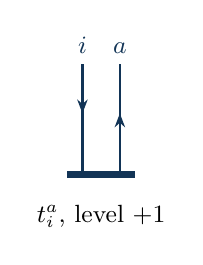
\begin{tikzpicture}[fcidiagram,scale=1.5,dlab/.style={font=\small}]
    \draw[amp] (-0.40,0) -- (0.40,0);
    \draw[hline] (-0.22,0) -- (-0.22,1.3) node[dlab,above] {$i$};
    \draw[pline] (0.22,0) -- (0.22,1.3) node[dlab,above] {$a$};
    \node[dlab,below] at (0.00,-0.25) {$t_i^a$, level $+1$};
\end{tikzpicture}
\hspace{1em}
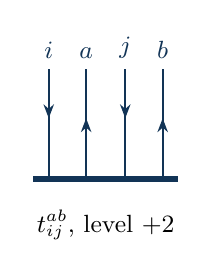
\begin{tikzpicture}[fcidiagram,scale=1.5,dlab/.style={font=\small}]
    \draw[amp] (-0.40,0) -- (1.30,0);
    \draw[hline] (-0.22,0) -- (-0.22,1.3) node[dlab,above] {$i$};
    \draw[pline] (0.22,0) -- (0.22,1.3) node[dlab,above] {$a$};
    \draw[hline] (0.68,0) -- (0.68,1.3) node[dlab,above] {$j$};
    \draw[pline] (1.12,0) -- (1.12,1.3) node[dlab,above] {$b$};
    \node[dlab,below] at (0.45,-0.25) {$t_{ij}^{ab}$, level $+2$};
\end{tikzpicture}

\vspace{0.8em}
\raggedright\footnotesize The new element: a bar with one vertex. All thirteen fragments of $H_N$ (week 47) are now in play, including those of odd level: $f_{ai}$, $f_{ia}$, $\as abcj$, $\as kaij$, $\as kacd$, $\as klcj$.
\column{0.7\textwidth}
\begin{block}{Drawing}
One fragment of $H_N$ on top; below it zero to four bars ($T_1$ or $T_2$), each attached to the fragment by at least one line; no lines between bars; the open lines are those of the projection ($i,a$ for the singles, $i,j,a,b$ for the doubles).
\end{block}
\begin{block}{Reading (unchanged from week 47)}
\begin{enumerate}
\item Sum over internal labels. Cross: $f_{\text{out},\text{in}}$; interaction: $\as{\text{left out}}{\text{right out}}{\text{left in}}{\text{right in}}$; bars: $t_i^a$, $t_{ij}^{ab}$.
\item Sign $(-1)^{h+l}$: hole lines and loops (external lines closed through the bra).
\item $\tfrac12$ for each pair of equivalent lines and each pair of equivalent vertices.
\item $P(ij)$, $P(ab)$ for external lines leaving different operators.
\end{enumerate}
\end{block}
\end{columns}
\vspace{0.4em}
Two $T_1$ bars attached to the same fragment in the same way are equivalent vertices: the $\tfrac1{2!}$, $\tfrac1{3!}$, $\tfrac1{4!}$ of the exponential, mostly cancelled by the number of ways of attaching identical bars.
\end{frame}

\begin{frame}[shrink=6]{The energy: three diagrams}
\small
\begin{center}
\begin{tabular}{@{}c@{\hspace{5em}}c@{\hspace{5em}}c@{}}
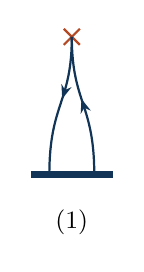
\begin{tikzpicture}[fcidiagram,baseline={(0,0)},dlab/.style={font=\small},scale=1.8]
    \draw[amp] (-0.40,0) -- (0.40,0);
    \node[fvtx] (h0) at (0.00,1.35) {};
    \draw[hline] (-0.22,0) .. controls (-0.22,0.7) and (0.00,0.7) .. (h0.center);
    \draw[pline] (0.22,0) .. controls (0.22,0.7) and (0.00,0.7) .. (h0.center);
    \node[dlab,below] at (0.00,-0.25) {(1)};
\end{tikzpicture} &
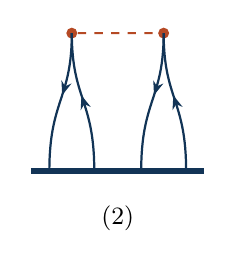
\begin{tikzpicture}[fcidiagram,baseline={(0,0)},dlab/.style={font=\small},scale=1.8]
    \draw[amp] (-0.40,0) -- (1.30,0);
    \node[vtx] (h0) at (0.00,1.35) {}; \node[vtx] (h1) at (0.90,1.35) {}; \draw[vint] (h0) -- (h1);
    \draw[hline] (-0.22,0) .. controls (-0.22,0.7) and (0.00,0.7) .. (h0.center);
    \draw[pline] (0.22,0) .. controls (0.22,0.7) and (0.00,0.7) .. (h0.center);
    \draw[hline] (0.68,0) .. controls (0.68,0.7) and (0.90,0.7) .. (h1.center);
    \draw[pline] (1.12,0) .. controls (1.12,0.7) and (0.90,0.7) .. (h1.center);
    \node[dlab,below] at (0.45,-0.25) {(2)};
\end{tikzpicture} &
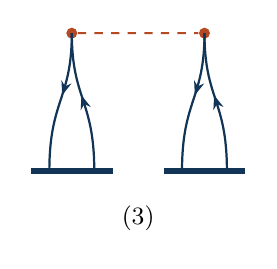
\begin{tikzpicture}[fcidiagram,baseline={(0,0)},dlab/.style={font=\small},scale=1.8]
    \draw[amp] (-0.40,0) -- (0.40,0);
    \draw[amp] (0.90,0) -- (1.70,0);
    \node[vtx] (h0) at (0.00,1.35) {}; \node[vtx] (h1) at (1.30,1.35) {}; \draw[vint] (h0) -- (h1);
    \draw[hline] (-0.22,0) .. controls (-0.22,0.7) and (0.00,0.7) .. (h0.center);
    \draw[pline] (0.22,0) .. controls (0.22,0.7) and (0.00,0.7) .. (h0.center);
    \draw[hline] (1.08,0) .. controls (1.08,0.7) and (1.30,0.7) .. (h1.center);
    \draw[pline] (1.52,0) .. controls (1.52,0.7) and (1.30,0.7) .. (h1.center);
    \node[dlab,below] at (0.65,-0.25) {(3)};
\end{tikzpicture}
\end{tabular}
\end{center}
\begin{columns}[T]
\column{0.32\textwidth}
\textbf{(1)} $f_{ia}$ closes a single. One hole line, one loop: $+$.
\[
 +\sum_{ia}f_{ia}\,t_i^a
\]
Zero in a Hartree-Fock basis.
\column{0.32\textwidth}
\textbf{(2)} $\as ijab$ closes a double. $h=2$, $l=2$; two pairs of equivalent lines.
\[
 +\frac14\sum_{ijab}\as ijab\,t_{ij}^{ab}
\]
The CCD energy.
\column{0.36\textwidth}
\textbf{(3)} $\as ijab$ closes two singles. $h=2$, $l=2$; no equivalent lines, but two equivalent vertices.
\[
 +\frac12\sum_{ijab}\as ijab\,t_i^at_j^b
\]
\end{columns}
\vspace{0.6em}
Diagram (3) is diagram (2) with the bar cut in two: wherever a $T_2$ bar is attached by both vertices, two $T_1$ bars can take its place. This is the combination $\tau_{ij}^{ab}=t_{ij}^{ab}+t_i^at_j^b-t_i^bt_j^a$ at work; analytically, (1) and (3) are $\tilde E_{\rm ref}-\Eref$.
\end{frame}

\begin{frame}[shrink=3]{The singles equation: fourteen diagrams}
\begin{center}
\begin{tabular}{@{}c@{\hspace{1.1em}}c@{\hspace{1.1em}}c@{\hspace{1.1em}}c@{\hspace{1.1em}}c@{\hspace{1.1em}}c@{\hspace{1.1em}}c@{}}
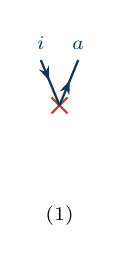
\begin{tikzpicture}[fcidiagram,baseline={(0,0)},scale=1.0]
    \node[fvtx] (h0) at (0.00,1.35) {};
    \draw[pline] (h0.center) -- (0.33,2.15) node[dlab,above] {$a$};
    \draw[hline] (h0.center) -- (-0.33,2.15) node[dlab,above] {$i$};
    \node[dlab,below] at (0.00,-0.25) {(1)};
\end{tikzpicture} &
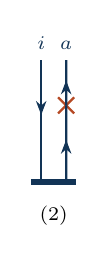
\begin{tikzpicture}[fcidiagram,baseline={(0,0)},scale=1.0]
    \draw[amp] (-0.40,0) -- (0.40,0);
    \node[fvtx] (h0) at (0.22,1.35) {};
    \draw[pline] (h0.center) -- (0.22,2.15) node[dlab,above] {$a$};
    \draw[pline] (0.22,0) .. controls (0.22,0.7) and (0.22,0.7) .. (h0.center);
    \draw[hline] (-0.22,0) -- (-0.22,2.15) node[dlab,above] {$i$};
    \node[dlab,below] at (0.00,-0.25) {(2)};
\end{tikzpicture} &
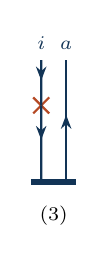
\begin{tikzpicture}[fcidiagram,baseline={(0,0)},scale=1.0]
    \draw[amp] (-0.40,0) -- (0.40,0);
    \node[fvtx] (h0) at (-0.22,1.35) {};
    \draw[hline] (-0.22,0) .. controls (-0.22,0.7) and (-0.22,0.7) .. (h0.center);
    \draw[hline] (h0.center) -- (-0.22,2.15) node[dlab,above] {$i$};
    \draw[pline] (0.22,0) -- (0.22,2.15) node[dlab,above] {$a$};
    \node[dlab,below] at (0.00,-0.25) {(3)};
\end{tikzpicture} &
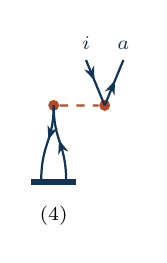
\begin{tikzpicture}[fcidiagram,baseline={(0,0)},scale=1.0]
    \draw[amp] (-0.40,0) -- (0.40,0);
    \node[vtx] (h0) at (0.00,1.35) {}; \node[vtx] (h1) at (0.90,1.35) {}; \draw[vint] (h0) -- (h1);
    \draw[hline] (-0.22,0) .. controls (-0.22,0.7) and (0.00,0.7) .. (h0.center);
    \draw[pline] (0.22,0) .. controls (0.22,0.7) and (0.00,0.7) .. (h0.center);
    \draw[pline] (h1.center) -- (1.23,2.15) node[dlab,above] {$a$};
    \draw[hline] (h1.center) -- (0.57,2.15) node[dlab,above] {$i$};
    \node[dlab,below] at (0.00,-0.25) {(4)};
\end{tikzpicture} &
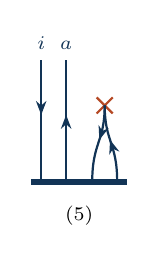
\begin{tikzpicture}[fcidiagram,baseline={(0,0)},scale=1.0]
    \draw[amp] (-0.40,0) -- (1.30,0);
    \node[fvtx] (h0) at (0.90,1.35) {};
    \draw[hline] (0.68,0) .. controls (0.68,0.7) and (0.90,0.7) .. (h0.center);
    \draw[pline] (1.12,0) .. controls (1.12,0.7) and (0.90,0.7) .. (h0.center);
    \draw[hline] (-0.22,0) -- (-0.22,2.15) node[dlab,above] {$i$};
    \draw[pline] (0.22,0) -- (0.22,2.15) node[dlab,above] {$a$};
    \node[dlab,below] at (0.45,-0.25) {(5)};
\end{tikzpicture} &
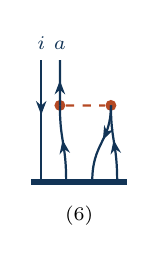
\begin{tikzpicture}[fcidiagram,baseline={(0,0)},scale=1.0]
    \draw[amp] (-0.40,0) -- (1.30,0);
    \node[vtx] (h0) at (0.11,1.35) {}; \node[vtx] (h1) at (1.01,1.35) {}; \draw[vint] (h0) -- (h1);
    \draw[pline] (h0.center) -- (0.11,2.15) node[dlab,above] {$a$};
    \draw[pline] (0.22,0) .. controls (0.22,0.7) and (0.11,0.7) .. (h0.center);
    \draw[hline] (0.68,0) .. controls (0.68,0.7) and (1.01,0.7) .. (h1.center);
    \draw[pline] (1.12,0) .. controls (1.12,0.7) and (1.01,0.7) .. (h1.center);
    \draw[hline] (-0.22,0) -- (-0.22,2.15) node[dlab,above] {$i$};
    \node[dlab,below] at (0.45,-0.25) {(6)};
\end{tikzpicture} &
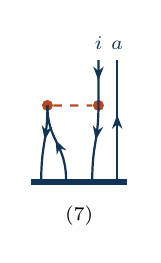
\begin{tikzpicture}[fcidiagram,baseline={(0,0)},scale=1.0]
    \draw[amp] (-0.40,0) -- (1.30,0);
    \node[vtx] (h0) at (-0.11,1.35) {}; \node[vtx] (h1) at (0.79,1.35) {}; \draw[vint] (h0) -- (h1);
    \draw[hline] (-0.22,0) .. controls (-0.22,0.7) and (-0.11,0.7) .. (h0.center);
    \draw[pline] (0.22,0) .. controls (0.22,0.7) and (-0.11,0.7) .. (h0.center);
    \draw[hline] (0.68,0) .. controls (0.68,0.7) and (0.79,0.7) .. (h1.center);
    \draw[hline] (h1.center) -- (0.79,2.15) node[dlab,above] {$i$};
    \draw[pline] (1.12,0) -- (1.12,2.15) node[dlab,above] {$a$};
    \node[dlab,below] at (0.45,-0.25) {(7)};
\end{tikzpicture}
\end{tabular}

\vspace{0.35em}
\begin{tabular}{@{}c@{\hspace{1.1em}}c@{\hspace{1.1em}}c@{\hspace{1.1em}}c@{\hspace{1.1em}}c@{\hspace{1.1em}}c@{\hspace{1.1em}}c@{}}
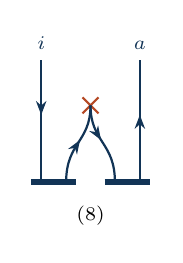
\begin{tikzpicture}[fcidiagram,baseline={(0,0)},scale=1.0]
    \draw[amp] (-0.40,0) -- (0.40,0);
    \draw[amp] (0.90,0) -- (1.70,0);
    \node[fvtx] (h0) at (0.65,1.35) {};
    \draw[hline] (1.08,0) .. controls (1.08,0.7) and (0.65,0.7) .. (h0.center);
    \draw[pline] (0.22,0) .. controls (0.22,0.7) and (0.65,0.7) .. (h0.center);
    \draw[hline] (-0.22,0) -- (-0.22,2.15) node[dlab,above] {$i$};
    \draw[pline] (1.52,0) -- (1.52,2.15) node[dlab,above] {$a$};
    \node[dlab,below] at (0.65,-0.25) {(8)};
\end{tikzpicture} &
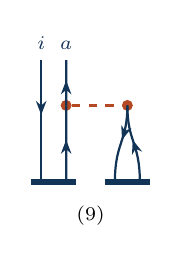
\begin{tikzpicture}[fcidiagram,baseline={(0,0)},scale=1.0]
    \draw[amp] (-0.40,0) -- (0.40,0);
    \draw[amp] (0.90,0) -- (1.70,0);
    \node[vtx] (h0) at (0.22,1.35) {}; \node[vtx] (h1) at (1.30,1.35) {}; \draw[vint] (h0) -- (h1);
    \draw[pline] (h0.center) -- (0.22,2.15) node[dlab,above] {$a$};
    \draw[pline] (0.22,0) .. controls (0.22,0.7) and (0.22,0.7) .. (h0.center);
    \draw[hline] (1.08,0) .. controls (1.08,0.7) and (1.30,0.7) .. (h1.center);
    \draw[pline] (1.52,0) .. controls (1.52,0.7) and (1.30,0.7) .. (h1.center);
    \draw[hline] (-0.22,0) -- (-0.22,2.15) node[dlab,above] {$i$};
    \node[dlab,below] at (0.65,-0.25) {(9)};
\end{tikzpicture} &
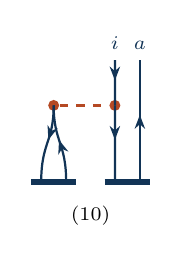
\begin{tikzpicture}[fcidiagram,baseline={(0,0)},scale=1.0]
    \draw[amp] (-0.40,0) -- (0.40,0);
    \draw[amp] (0.90,0) -- (1.70,0);
    \node[vtx] (h0) at (0.00,1.35) {}; \node[vtx] (h1) at (1.08,1.35) {}; \draw[vint] (h0) -- (h1);
    \draw[hline] (-0.22,0) .. controls (-0.22,0.7) and (0.00,0.7) .. (h0.center);
    \draw[pline] (0.22,0) .. controls (0.22,0.7) and (0.00,0.7) .. (h0.center);
    \draw[hline] (1.08,0) .. controls (1.08,0.7) and (1.08,0.7) .. (h1.center);
    \draw[hline] (h1.center) -- (1.08,2.15) node[dlab,above] {$i$};
    \draw[pline] (1.52,0) -- (1.52,2.15) node[dlab,above] {$a$};
    \node[dlab,below] at (0.65,-0.25) {(10)};
\end{tikzpicture} &
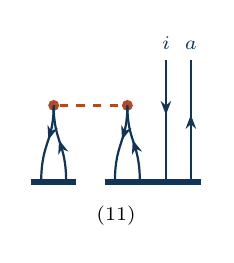
\begin{tikzpicture}[fcidiagram,baseline={(0,0)},scale=1.0]
    \draw[amp] (-0.40,0) -- (0.40,0);
    \draw[amp] (0.90,0) -- (2.60,0);
    \node[vtx] (h0) at (0.00,1.35) {}; \node[vtx] (h1) at (1.30,1.35) {}; \draw[vint] (h0) -- (h1);
    \draw[hline] (-0.22,0) .. controls (-0.22,0.7) and (0.00,0.7) .. (h0.center);
    \draw[pline] (0.22,0) .. controls (0.22,0.7) and (0.00,0.7) .. (h0.center);
    \draw[hline] (1.08,0) .. controls (1.08,0.7) and (1.30,0.7) .. (h1.center);
    \draw[pline] (1.52,0) .. controls (1.52,0.7) and (1.30,0.7) .. (h1.center);
    \draw[hline] (1.98,0) -- (1.98,2.15) node[dlab,above] {$i$};
    \draw[pline] (2.42,0) -- (2.42,2.15) node[dlab,above] {$a$};
    \node[dlab,below] at (1.10,-0.25) {(11)};
\end{tikzpicture} &
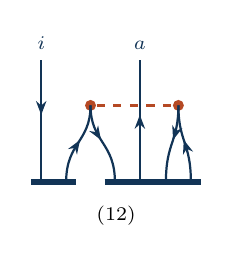
\begin{tikzpicture}[fcidiagram,baseline={(0,0)},scale=1.0]
    \draw[amp] (-0.40,0) -- (0.40,0);
    \draw[amp] (0.90,0) -- (2.60,0);
    \node[vtx] (h0) at (0.65,1.35) {}; \node[vtx] (h1) at (2.20,1.35) {}; \draw[vint] (h0) -- (h1);
    \draw[hline] (1.08,0) .. controls (1.08,0.7) and (0.65,0.7) .. (h0.center);
    \draw[pline] (0.22,0) .. controls (0.22,0.7) and (0.65,0.7) .. (h0.center);
    \draw[hline] (1.98,0) .. controls (1.98,0.7) and (2.20,0.7) .. (h1.center);
    \draw[pline] (2.42,0) .. controls (2.42,0.7) and (2.20,0.7) .. (h1.center);
    \draw[hline] (-0.22,0) -- (-0.22,2.15) node[dlab,above] {$i$};
    \draw[pline] (1.52,0) -- (1.52,2.15) node[dlab,above] {$a$};
    \node[dlab,below] at (1.10,-0.25) {(12)};
\end{tikzpicture} &
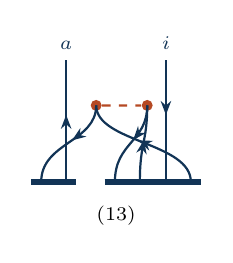
\begin{tikzpicture}[fcidiagram,baseline={(0,0)},scale=1.0]
    \draw[amp] (-0.40,0) -- (0.40,0);
    \draw[amp] (0.90,0) -- (2.60,0);
    \node[vtx] (h0) at (0.75,1.35) {}; \node[vtx] (h1) at (1.65,1.35) {}; \draw[vint] (h0) -- (h1);
    \draw[hline] (-0.22,0) .. controls (-0.22,0.7) and (0.75,0.7) .. (h0.center);
    \draw[pline] (2.42,0) .. controls (2.42,0.7) and (0.75,0.7) .. (h0.center);
    \draw[hline] (1.08,0) .. controls (1.08,0.7) and (1.65,0.7) .. (h1.center);
    \draw[pline] (1.52,0) .. controls (1.52,0.7) and (1.65,0.7) .. (h1.center);
    \draw[pline] (0.22,0) -- (0.22,2.15) node[dlab,above] {$a$};
    \draw[hline] (1.98,0) -- (1.98,2.15) node[dlab,above] {$i$};
    \node[dlab,below] at (1.10,-0.25) {(13)};
\end{tikzpicture} &
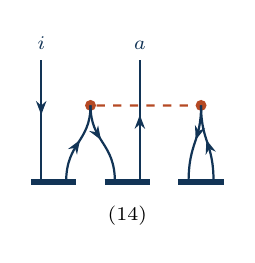
\begin{tikzpicture}[fcidiagram,baseline={(0,0)},scale=1.0]
    \draw[amp] (-0.40,0) -- (0.40,0);
    \draw[amp] (0.90,0) -- (1.70,0);
    \draw[amp] (2.20,0) -- (3.00,0);
    \node[vtx] (h0) at (0.65,1.35) {}; \node[vtx] (h1) at (2.60,1.35) {}; \draw[vint] (h0) -- (h1);
    \draw[hline] (1.08,0) .. controls (1.08,0.7) and (0.65,0.7) .. (h0.center);
    \draw[pline] (0.22,0) .. controls (0.22,0.7) and (0.65,0.7) .. (h0.center);
    \draw[hline] (2.38,0) .. controls (2.38,0.7) and (2.60,0.7) .. (h1.center);
    \draw[pline] (2.82,0) .. controls (2.82,0.7) and (2.60,0.7) .. (h1.center);
    \draw[hline] (-0.22,0) -- (-0.22,2.15) node[dlab,above] {$i$};
    \draw[pline] (1.52,0) -- (1.52,2.15) node[dlab,above] {$a$};
    \node[dlab,below] at (1.30,-0.25) {(14)};
\end{tikzpicture}
\end{tabular}
\end{center}
\footnotesize
(1) the driving term $f_{ai}$; (2)--(4) one $T_1$; (5)--(7) one $T_2$, attached by two or three lines; (8)--(10) two $T_1$; (11)--(13) $T_1T_2$; (14) three $T_1$. The dressing of lecture 1: (2), (3), (4), (8), (9), (10), (14) are (1) with $T_1$ bars hung on its lines -- together $\ft_{ai}$; (11) is (5), (13) is (6) and (12) is (7), each with one more $T_1$.
\end{frame}

\begin{frame}{The singles equation, read off}
\small
\begin{align*}
0={}&f_{ai}+f_{ae}t_i^e-f_{mi}t_m^a+\as maei\,t_m^e
 +f_{me}t_{im}^{ae}+\tfrac12\as amef\,t_{im}^{ef}-\tfrac12\as mnei\,t_{mn}^{ea}\\
 &-f_{me}t_i^et_m^a+\as amef\,t_i^et_m^f-\as mnei\,t_m^et_n^a
 +\as mnef\,t_m^et_{ni}^{fa}-\tfrac12\as mnef\,t_i^et_{mn}^{af}-\tfrac12\as mnef\,t_n^at_{mi}^{ef}\\
 &-\as mnef\,t_i^et_m^at_n^f
\end{align*}
(terms in the order of the diagrams; internal labels $m,n$ holes and $e,f$ particles, summed).
\begin{columns}[T]
\column{0.5\textwidth}
\textbf{Diagram (3)}, $-f_{mi}t_m^a$: the cross sits on the hole line, which runs from the external $i$ through the cross to the bar as $m$. Hole lines $m,i$: $h=2$. One loop (through the bra). Sign $(-1)^{2+1}=-$.

\vspace{0.4em}
\textbf{Diagram (4)}, $+\as maei t_m^e$: the single is annihilated at one vertex and the pair $(a,i)$ created at the other. $h=2$, $l=2$: $+$. The ring diagram of the singles.
\column{0.5\textwidth}
\textbf{Diagram (7)}, $-\tfrac12\as mnei t_{mn}^{ea}$: hole lines $m,n,i$: $h=3$; loops $(m,e)$ and the external one: $l=2$; sign $-$. The lines $m,n$ are equivalent: $\tfrac12$.

\vspace{0.4em}
\textbf{Diagrams (6), (7)} are how doubles induce singles: three lines of the bar enter $\as amef$ or $\as mnei$. In a Hartree-Fock basis they are the leading terms: $t_1$ starts at second order.
\end{columns}
\end{frame}

\begin{frame}[shrink=16]{The doubles equation: diagrams (1)--(16)}
\begin{center}
\begin{tabular}{@{}c@{\hspace{1.2em}}c@{\hspace{1.2em}}c@{\hspace{1.2em}}c@{\hspace{1.2em}}c@{\hspace{1.2em}}c@{}}
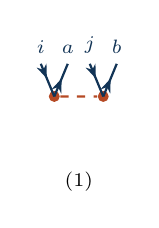
\begin{tikzpicture}[fcidiagram,baseline={(0,0)},scale=0.72]
    \node[vtx] (h0) at (-0.60,1.35) {}; \node[vtx] (h1) at (0.60,1.35) {}; \draw[vint] (h0) -- (h1);
    \draw[pline] (h0.center) -- (-0.27,2.15) node[dlab,above] {$a$};
    \draw[hline] (h0.center) -- (-0.93,2.15) node[dlab,above] {$i$};
    \draw[pline] (h1.center) -- (0.93,2.15) node[dlab,above] {$b$};
    \draw[hline] (h1.center) -- (0.27,2.15) node[dlab,above] {$j$};
    \node[dlab,below] at (0.00,-0.25) {(1)};
\end{tikzpicture} &
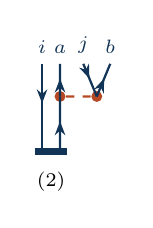
\begin{tikzpicture}[fcidiagram,baseline={(0,0)},scale=0.72]
    \draw[amp] (-0.40,0) -- (0.40,0);
    \node[vtx] (h0) at (0.22,1.35) {}; \node[vtx] (h1) at (1.12,1.35) {}; \draw[vint] (h0) -- (h1);
    \draw[pline] (h0.center) -- (0.22,2.15) node[dlab,above] {$a$};
    \draw[pline] (0.22,0) .. controls (0.22,0.7) and (0.22,0.7) .. (h0.center);
    \draw[pline] (h1.center) -- (1.45,2.15) node[dlab,above] {$b$};
    \draw[hline] (h1.center) -- (0.79,2.15) node[dlab,above] {$j$};
    \draw[hline] (-0.22,0) -- (-0.22,2.15) node[dlab,above] {$i$};
    \node[dlab,below] at (0.00,-0.25) {(2)};
\end{tikzpicture} &
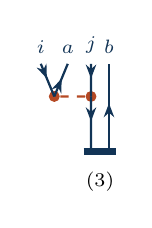
\begin{tikzpicture}[fcidiagram,baseline={(0,0)},scale=0.72]
    \draw[amp] (-0.40,0) -- (0.40,0);
    \node[vtx] (h0) at (-1.12,1.35) {}; \node[vtx] (h1) at (-0.22,1.35) {}; \draw[vint] (h0) -- (h1);
    \draw[pline] (h0.center) -- (-0.79,2.15) node[dlab,above] {$a$};
    \draw[hline] (h0.center) -- (-1.45,2.15) node[dlab,above] {$i$};
    \draw[hline] (-0.22,0) .. controls (-0.22,0.7) and (-0.22,0.7) .. (h1.center);
    \draw[hline] (h1.center) -- (-0.22,2.15) node[dlab,above] {$j$};
    \draw[pline] (0.22,0) -- (0.22,2.15) node[dlab,above] {$b$};
    \node[dlab,below] at (0.00,-0.25) {(3)};
\end{tikzpicture} &
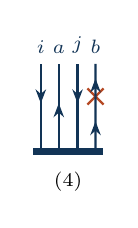
\begin{tikzpicture}[fcidiagram,baseline={(0,0)},scale=0.72]
    \draw[amp] (-0.40,0) -- (1.30,0);
    \node[fvtx] (h0) at (1.12,1.35) {};
    \draw[pline] (h0.center) -- (1.12,2.15) node[dlab,above] {$b$};
    \draw[pline] (1.12,0) .. controls (1.12,0.7) and (1.12,0.7) .. (h0.center);
    \draw[hline] (-0.22,0) -- (-0.22,2.15) node[dlab,above] {$i$};
    \draw[pline] (0.22,0) -- (0.22,2.15) node[dlab,above] {$a$};
    \draw[hline] (0.68,0) -- (0.68,2.15) node[dlab,above] {$j$};
    \node[dlab,below] at (0.45,-0.25) {(4)};
\end{tikzpicture} &
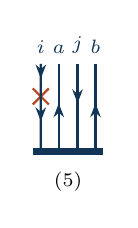
\begin{tikzpicture}[fcidiagram,baseline={(0,0)},scale=0.72]
    \draw[amp] (-0.40,0) -- (1.30,0);
    \node[fvtx] (h0) at (-0.22,1.35) {};
    \draw[hline] (-0.22,0) .. controls (-0.22,0.7) and (-0.22,0.7) .. (h0.center);
    \draw[hline] (h0.center) -- (-0.22,2.15) node[dlab,above] {$i$};
    \draw[pline] (0.22,0) -- (0.22,2.15) node[dlab,above] {$a$};
    \draw[hline] (0.68,0) -- (0.68,2.15) node[dlab,above] {$j$};
    \draw[pline] (1.12,0) -- (1.12,2.15) node[dlab,above] {$b$};
    \node[dlab,below] at (0.45,-0.25) {(5)};
\end{tikzpicture} &
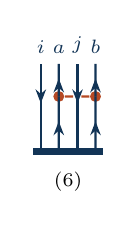
\begin{tikzpicture}[fcidiagram,baseline={(0,0)},scale=0.72]
    \draw[amp] (-0.40,0) -- (1.30,0);
    \node[vtx] (h0) at (0.22,1.35) {}; \node[vtx] (h1) at (1.12,1.35) {}; \draw[vint] (h0) -- (h1);
    \draw[pline] (h0.center) -- (0.22,2.15) node[dlab,above] {$a$};
    \draw[pline] (0.22,0) .. controls (0.22,0.7) and (0.22,0.7) .. (h0.center);
    \draw[pline] (h1.center) -- (1.12,2.15) node[dlab,above] {$b$};
    \draw[pline] (1.12,0) .. controls (1.12,0.7) and (1.12,0.7) .. (h1.center);
    \draw[hline] (-0.22,0) -- (-0.22,2.15) node[dlab,above] {$i$};
    \draw[hline] (0.68,0) -- (0.68,2.15) node[dlab,above] {$j$};
    \node[dlab,below] at (0.45,-0.25) {(6)};
\end{tikzpicture}
\end{tabular}

\vspace{0.35em}
\begin{tabular}{@{}c@{\hspace{1.2em}}c@{\hspace{1.2em}}c@{\hspace{1.2em}}c@{\hspace{1.2em}}c@{\hspace{1.2em}}c@{}}
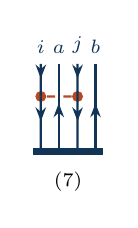
\begin{tikzpicture}[fcidiagram,baseline={(0,0)},scale=0.72]
    \draw[amp] (-0.40,0) -- (1.30,0);
    \node[vtx] (h0) at (-0.22,1.35) {}; \node[vtx] (h1) at (0.68,1.35) {}; \draw[vint] (h0) -- (h1);
    \draw[hline] (-0.22,0) .. controls (-0.22,0.7) and (-0.22,0.7) .. (h0.center);
    \draw[hline] (h0.center) -- (-0.22,2.15) node[dlab,above] {$i$};
    \draw[hline] (0.68,0) .. controls (0.68,0.7) and (0.68,0.7) .. (h1.center);
    \draw[hline] (h1.center) -- (0.68,2.15) node[dlab,above] {$j$};
    \draw[pline] (0.22,0) -- (0.22,2.15) node[dlab,above] {$a$};
    \draw[pline] (1.12,0) -- (1.12,2.15) node[dlab,above] {$b$};
    \node[dlab,below] at (0.45,-0.25) {(7)};
\end{tikzpicture} &
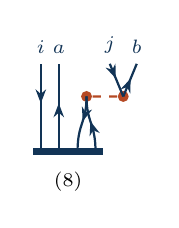
\begin{tikzpicture}[fcidiagram,baseline={(0,0)},scale=0.72]
    \draw[amp] (-0.40,0) -- (1.30,0);
    \node[vtx] (h0) at (0.90,1.35) {}; \node[vtx] (h1) at (1.80,1.35) {}; \draw[vint] (h0) -- (h1);
    \draw[hline] (0.68,0) .. controls (0.68,0.7) and (0.90,0.7) .. (h0.center);
    \draw[pline] (1.12,0) .. controls (1.12,0.7) and (0.90,0.7) .. (h0.center);
    \draw[pline] (h1.center) -- (2.13,2.15) node[dlab,above] {$b$};
    \draw[hline] (h1.center) -- (1.47,2.15) node[dlab,above] {$j$};
    \draw[hline] (-0.22,0) -- (-0.22,2.15) node[dlab,above] {$i$};
    \draw[pline] (0.22,0) -- (0.22,2.15) node[dlab,above] {$a$};
    \node[dlab,below] at (0.45,-0.25) {(8)};
\end{tikzpicture} &
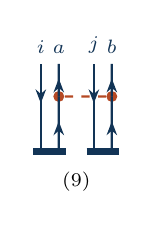
\begin{tikzpicture}[fcidiagram,baseline={(0,0)},scale=0.72]
    \draw[amp] (-0.40,0) -- (0.40,0);
    \draw[amp] (0.90,0) -- (1.70,0);
    \node[vtx] (h0) at (0.22,1.35) {}; \node[vtx] (h1) at (1.52,1.35) {}; \draw[vint] (h0) -- (h1);
    \draw[pline] (h0.center) -- (0.22,2.15) node[dlab,above] {$a$};
    \draw[pline] (0.22,0) .. controls (0.22,0.7) and (0.22,0.7) .. (h0.center);
    \draw[pline] (h1.center) -- (1.52,2.15) node[dlab,above] {$b$};
    \draw[pline] (1.52,0) .. controls (1.52,0.7) and (1.52,0.7) .. (h1.center);
    \draw[hline] (-0.22,0) -- (-0.22,2.15) node[dlab,above] {$i$};
    \draw[hline] (1.08,0) -- (1.08,2.15) node[dlab,above] {$j$};
    \node[dlab,below] at (0.65,-0.25) {(9)};
\end{tikzpicture} &
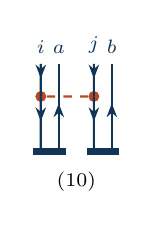
\begin{tikzpicture}[fcidiagram,baseline={(0,0)},scale=0.72]
    \draw[amp] (-0.40,0) -- (0.40,0);
    \draw[amp] (0.90,0) -- (1.70,0);
    \node[vtx] (h0) at (-0.22,1.35) {}; \node[vtx] (h1) at (1.08,1.35) {}; \draw[vint] (h0) -- (h1);
    \draw[hline] (-0.22,0) .. controls (-0.22,0.7) and (-0.22,0.7) .. (h0.center);
    \draw[hline] (h0.center) -- (-0.22,2.15) node[dlab,above] {$i$};
    \draw[hline] (1.08,0) .. controls (1.08,0.7) and (1.08,0.7) .. (h1.center);
    \draw[hline] (h1.center) -- (1.08,2.15) node[dlab,above] {$j$};
    \draw[pline] (0.22,0) -- (0.22,2.15) node[dlab,above] {$a$};
    \draw[pline] (1.52,0) -- (1.52,2.15) node[dlab,above] {$b$};
    \node[dlab,below] at (0.65,-0.25) {(10)};
\end{tikzpicture} &
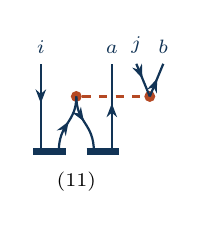
\begin{tikzpicture}[fcidiagram,baseline={(0,0)},scale=0.72]
    \draw[amp] (-0.40,0) -- (0.40,0);
    \draw[amp] (0.90,0) -- (1.70,0);
    \node[vtx] (h0) at (0.65,1.35) {}; \node[vtx] (h1) at (2.45,1.35) {}; \draw[vint] (h0) -- (h1);
    \draw[hline] (1.08,0) .. controls (1.08,0.7) and (0.65,0.7) .. (h0.center);
    \draw[pline] (0.22,0) .. controls (0.22,0.7) and (0.65,0.7) .. (h0.center);
    \draw[pline] (h1.center) -- (2.78,2.15) node[dlab,above] {$b$};
    \draw[hline] (h1.center) -- (2.12,2.15) node[dlab,above] {$j$};
    \draw[hline] (-0.22,0) -- (-0.22,2.15) node[dlab,above] {$i$};
    \draw[pline] (1.52,0) -- (1.52,2.15) node[dlab,above] {$a$};
    \node[dlab,below] at (0.65,-0.25) {(11)};
\end{tikzpicture} &
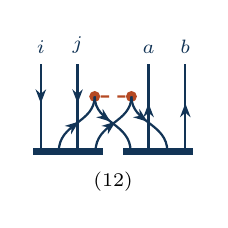
\begin{tikzpicture}[fcidiagram,baseline={(0,0)},scale=0.72]
    \draw[amp] (-0.40,0) -- (1.30,0);
    \draw[amp] (1.80,0) -- (3.50,0);
    \node[vtx] (h0) at (1.10,1.35) {}; \node[vtx] (h1) at (2.00,1.35) {}; \draw[vint] (h0) -- (h1);
    \draw[hline] (1.98,0) .. controls (1.98,0.7) and (1.10,0.7) .. (h0.center);
    \draw[pline] (0.22,0) .. controls (0.22,0.7) and (1.10,0.7) .. (h0.center);
    \draw[hline] (2.88,0) .. controls (2.88,0.7) and (2.00,0.7) .. (h1.center);
    \draw[pline] (1.12,0) .. controls (1.12,0.7) and (2.00,0.7) .. (h1.center);
    \draw[hline] (-0.22,0) -- (-0.22,2.15) node[dlab,above] {$i$};
    \draw[hline] (0.68,0) -- (0.68,2.15) node[dlab,above] {$j$};
    \draw[pline] (2.42,0) -- (2.42,2.15) node[dlab,above] {$a$};
    \draw[pline] (3.32,0) -- (3.32,2.15) node[dlab,above] {$b$};
    \node[dlab,below] at (1.55,-0.25) {(12)};
\end{tikzpicture}
\end{tabular}

\vspace{0.35em}
\begin{tabular}{@{}c@{\hspace{1.2em}}c@{\hspace{1.2em}}c@{\hspace{1.2em}}c@{}}
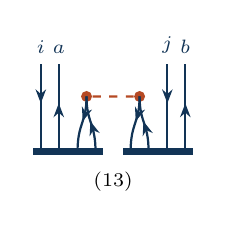
\begin{tikzpicture}[fcidiagram,baseline={(0,0)},scale=0.72]
    \draw[amp] (-0.40,0) -- (1.30,0);
    \draw[amp] (1.80,0) -- (3.50,0);
    \node[vtx] (h0) at (0.90,1.35) {}; \node[vtx] (h1) at (2.20,1.35) {}; \draw[vint] (h0) -- (h1);
    \draw[hline] (0.68,0) .. controls (0.68,0.7) and (0.90,0.7) .. (h0.center);
    \draw[pline] (1.12,0) .. controls (1.12,0.7) and (0.90,0.7) .. (h0.center);
    \draw[hline] (1.98,0) .. controls (1.98,0.7) and (2.20,0.7) .. (h1.center);
    \draw[pline] (2.42,0) .. controls (2.42,0.7) and (2.20,0.7) .. (h1.center);
    \draw[hline] (-0.22,0) -- (-0.22,2.15) node[dlab,above] {$i$};
    \draw[pline] (0.22,0) -- (0.22,2.15) node[dlab,above] {$a$};
    \draw[hline] (2.88,0) -- (2.88,2.15) node[dlab,above] {$j$};
    \draw[pline] (3.32,0) -- (3.32,2.15) node[dlab,above] {$b$};
    \node[dlab,below] at (1.55,-0.25) {(13)};
\end{tikzpicture} &
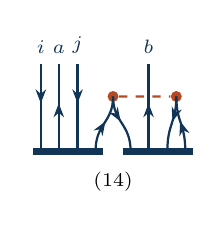
\begin{tikzpicture}[fcidiagram,baseline={(0,0)},scale=0.72]
    \draw[amp] (-0.40,0) -- (1.30,0);
    \draw[amp] (1.80,0) -- (3.50,0);
    \node[vtx] (h0) at (1.55,1.35) {}; \node[vtx] (h1) at (3.10,1.35) {}; \draw[vint] (h0) -- (h1);
    \draw[hline] (1.98,0) .. controls (1.98,0.7) and (1.55,0.7) .. (h0.center);
    \draw[pline] (1.12,0) .. controls (1.12,0.7) and (1.55,0.7) .. (h0.center);
    \draw[hline] (2.88,0) .. controls (2.88,0.7) and (3.10,0.7) .. (h1.center);
    \draw[pline] (3.32,0) .. controls (3.32,0.7) and (3.10,0.7) .. (h1.center);
    \draw[hline] (-0.22,0) -- (-0.22,2.15) node[dlab,above] {$i$};
    \draw[pline] (0.22,0) -- (0.22,2.15) node[dlab,above] {$a$};
    \draw[hline] (0.68,0) -- (0.68,2.15) node[dlab,above] {$j$};
    \draw[pline] (2.42,0) -- (2.42,2.15) node[dlab,above] {$b$};
    \node[dlab,below] at (1.55,-0.25) {(14)};
\end{tikzpicture} &
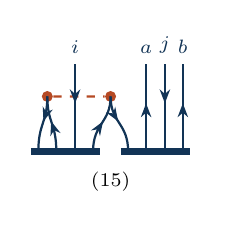
\begin{tikzpicture}[fcidiagram,baseline={(0,0)},scale=0.72]
    \draw[amp] (-0.40,0) -- (1.30,0);
    \draw[amp] (1.80,0) -- (3.50,0);
    \node[vtx] (h0) at (0.00,1.35) {}; \node[vtx] (h1) at (1.55,1.35) {}; \draw[vint] (h0) -- (h1);
    \draw[hline] (-0.22,0) .. controls (-0.22,0.7) and (0.00,0.7) .. (h0.center);
    \draw[pline] (0.22,0) .. controls (0.22,0.7) and (0.00,0.7) .. (h0.center);
    \draw[hline] (1.98,0) .. controls (1.98,0.7) and (1.55,0.7) .. (h1.center);
    \draw[pline] (1.12,0) .. controls (1.12,0.7) and (1.55,0.7) .. (h1.center);
    \draw[hline] (0.68,0) -- (0.68,2.15) node[dlab,above] {$i$};
    \draw[pline] (2.42,0) -- (2.42,2.15) node[dlab,above] {$a$};
    \draw[hline] (2.88,0) -- (2.88,2.15) node[dlab,above] {$j$};
    \draw[pline] (3.32,0) -- (3.32,2.15) node[dlab,above] {$b$};
    \node[dlab,below] at (1.55,-0.25) {(15)};
\end{tikzpicture} &
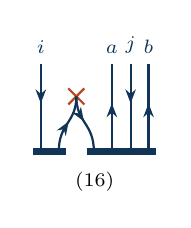
\begin{tikzpicture}[fcidiagram,baseline={(0,0)},scale=0.72]
    \draw[amp] (-0.40,0) -- (0.40,0);
    \draw[amp] (0.90,0) -- (2.60,0);
    \node[fvtx] (h0) at (0.65,1.35) {};
    \draw[hline] (1.08,0) .. controls (1.08,0.7) and (0.65,0.7) .. (h0.center);
    \draw[pline] (0.22,0) .. controls (0.22,0.7) and (0.65,0.7) .. (h0.center);
    \draw[hline] (-0.22,0) -- (-0.22,2.15) node[dlab,above] {$i$};
    \draw[pline] (1.52,0) -- (1.52,2.15) node[dlab,above] {$a$};
    \draw[hline] (1.98,0) -- (1.98,2.15) node[dlab,above] {$j$};
    \draw[pline] (2.42,0) -- (2.42,2.15) node[dlab,above] {$b$};
    \node[dlab,below] at (1.10,-0.25) {(16)};
\end{tikzpicture}
\end{tabular}
\end{center}
\footnotesize
(1) driving term; (2), (3) one $T_1$ on the level $+1$ fragments $\as abej$, $\as amij$; \textbf{(4)--(8) the linear CCD diagrams}: Fock, Fock, pp ladder, hh ladder, ring; (9)--(11) the ladders and the ring with the $T_2$ bar cut into two $T_1$; \textbf{(12)--(15) the quadratic CCD diagrams} $Q_a,Q_b,Q_c,Q_d$; (16) $f_{me}$ joining a $T_1$ and a $T_2$.
\end{frame}

\begin{frame}[shrink=19]{The doubles equation: diagrams (17)--(31)}
\begin{center}
\begin{tabular}{@{}c@{\hspace{1.6em}}c@{\hspace{1.6em}}c@{\hspace{1.6em}}c@{\hspace{1.6em}}c@{}}
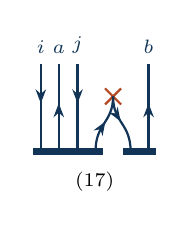
\begin{tikzpicture}[fcidiagram,baseline={(0,0)},scale=0.72]
    \draw[amp] (-0.40,0) -- (1.30,0);
    \draw[amp] (1.80,0) -- (2.60,0);
    \node[fvtx] (h0) at (1.55,1.35) {};
    \draw[hline] (1.98,0) .. controls (1.98,0.7) and (1.55,0.7) .. (h0.center);
    \draw[pline] (1.12,0) .. controls (1.12,0.7) and (1.55,0.7) .. (h0.center);
    \draw[hline] (-0.22,0) -- (-0.22,2.15) node[dlab,above] {$i$};
    \draw[pline] (0.22,0) -- (0.22,2.15) node[dlab,above] {$a$};
    \draw[hline] (0.68,0) -- (0.68,2.15) node[dlab,above] {$j$};
    \draw[pline] (2.42,0) -- (2.42,2.15) node[dlab,above] {$b$};
    \node[dlab,below] at (1.10,-0.25) {(17)};
\end{tikzpicture} &
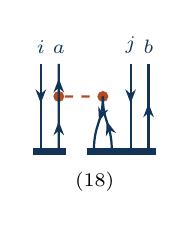
\begin{tikzpicture}[fcidiagram,baseline={(0,0)},scale=0.72]
    \draw[amp] (-0.40,0) -- (0.40,0);
    \draw[amp] (0.90,0) -- (2.60,0);
    \node[vtx] (h0) at (0.22,1.35) {}; \node[vtx] (h1) at (1.30,1.35) {}; \draw[vint] (h0) -- (h1);
    \draw[pline] (h0.center) -- (0.22,2.15) node[dlab,above] {$a$};
    \draw[pline] (0.22,0) .. controls (0.22,0.7) and (0.22,0.7) .. (h0.center);
    \draw[hline] (1.08,0) .. controls (1.08,0.7) and (1.30,0.7) .. (h1.center);
    \draw[pline] (1.52,0) .. controls (1.52,0.7) and (1.30,0.7) .. (h1.center);
    \draw[hline] (-0.22,0) -- (-0.22,2.15) node[dlab,above] {$i$};
    \draw[hline] (1.98,0) -- (1.98,2.15) node[dlab,above] {$j$};
    \draw[pline] (2.42,0) -- (2.42,2.15) node[dlab,above] {$b$};
    \node[dlab,below] at (1.10,-0.25) {(18)};
\end{tikzpicture} &
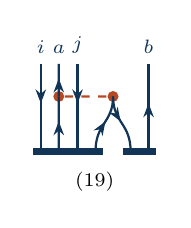
\begin{tikzpicture}[fcidiagram,baseline={(0,0)},scale=0.72]
    \draw[amp] (-0.40,0) -- (1.30,0);
    \draw[amp] (1.80,0) -- (2.60,0);
    \node[vtx] (h0) at (0.22,1.35) {}; \node[vtx] (h1) at (1.55,1.35) {}; \draw[vint] (h0) -- (h1);
    \draw[pline] (h0.center) -- (0.22,2.15) node[dlab,above] {$a$};
    \draw[pline] (0.22,0) .. controls (0.22,0.7) and (0.22,0.7) .. (h0.center);
    \draw[hline] (1.98,0) .. controls (1.98,0.7) and (1.55,0.7) .. (h1.center);
    \draw[pline] (1.12,0) .. controls (1.12,0.7) and (1.55,0.7) .. (h1.center);
    \draw[hline] (-0.22,0) -- (-0.22,2.15) node[dlab,above] {$i$};
    \draw[hline] (0.68,0) -- (0.68,2.15) node[dlab,above] {$j$};
    \draw[pline] (2.42,0) -- (2.42,2.15) node[dlab,above] {$b$};
    \node[dlab,below] at (1.10,-0.25) {(19)};
\end{tikzpicture} &
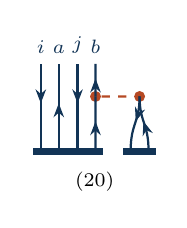
\begin{tikzpicture}[fcidiagram,baseline={(0,0)},scale=0.72]
    \draw[amp] (-0.40,0) -- (1.30,0);
    \draw[amp] (1.80,0) -- (2.60,0);
    \node[vtx] (h0) at (1.12,1.35) {}; \node[vtx] (h1) at (2.20,1.35) {}; \draw[vint] (h0) -- (h1);
    \draw[pline] (h0.center) -- (1.12,2.15) node[dlab,above] {$b$};
    \draw[pline] (1.12,0) .. controls (1.12,0.7) and (1.12,0.7) .. (h0.center);
    \draw[hline] (1.98,0) .. controls (1.98,0.7) and (2.20,0.7) .. (h1.center);
    \draw[pline] (2.42,0) .. controls (2.42,0.7) and (2.20,0.7) .. (h1.center);
    \draw[hline] (-0.22,0) -- (-0.22,2.15) node[dlab,above] {$i$};
    \draw[pline] (0.22,0) -- (0.22,2.15) node[dlab,above] {$a$};
    \draw[hline] (0.68,0) -- (0.68,2.15) node[dlab,above] {$j$};
    \node[dlab,below] at (1.10,-0.25) {(20)};
\end{tikzpicture} &
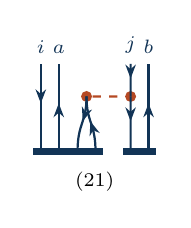
\begin{tikzpicture}[fcidiagram,baseline={(0,0)},scale=0.72]
    \draw[amp] (-0.40,0) -- (1.30,0);
    \draw[amp] (1.80,0) -- (2.60,0);
    \node[vtx] (h0) at (0.90,1.35) {}; \node[vtx] (h1) at (1.98,1.35) {}; \draw[vint] (h0) -- (h1);
    \draw[hline] (0.68,0) .. controls (0.68,0.7) and (0.90,0.7) .. (h0.center);
    \draw[pline] (1.12,0) .. controls (1.12,0.7) and (0.90,0.7) .. (h0.center);
    \draw[hline] (1.98,0) .. controls (1.98,0.7) and (1.98,0.7) .. (h1.center);
    \draw[hline] (h1.center) -- (1.98,2.15) node[dlab,above] {$j$};
    \draw[hline] (-0.22,0) -- (-0.22,2.15) node[dlab,above] {$i$};
    \draw[pline] (0.22,0) -- (0.22,2.15) node[dlab,above] {$a$};
    \draw[pline] (2.42,0) -- (2.42,2.15) node[dlab,above] {$b$};
    \node[dlab,below] at (1.10,-0.25) {(21)};
\end{tikzpicture}
\end{tabular}

\vspace{0.35em}
\begin{tabular}{@{}c@{\hspace{1.6em}}c@{\hspace{1.6em}}c@{\hspace{1.6em}}c@{\hspace{1.6em}}c@{}}
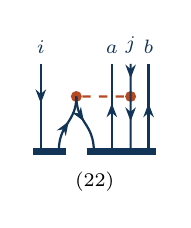
\begin{tikzpicture}[fcidiagram,baseline={(0,0)},scale=0.72]
    \draw[amp] (-0.40,0) -- (0.40,0);
    \draw[amp] (0.90,0) -- (2.60,0);
    \node[vtx] (h0) at (0.65,1.35) {}; \node[vtx] (h1) at (1.98,1.35) {}; \draw[vint] (h0) -- (h1);
    \draw[hline] (1.08,0) .. controls (1.08,0.7) and (0.65,0.7) .. (h0.center);
    \draw[pline] (0.22,0) .. controls (0.22,0.7) and (0.65,0.7) .. (h0.center);
    \draw[hline] (1.98,0) .. controls (1.98,0.7) and (1.98,0.7) .. (h1.center);
    \draw[hline] (h1.center) -- (1.98,2.15) node[dlab,above] {$j$};
    \draw[hline] (-0.22,0) -- (-0.22,2.15) node[dlab,above] {$i$};
    \draw[pline] (1.52,0) -- (1.52,2.15) node[dlab,above] {$a$};
    \draw[pline] (2.42,0) -- (2.42,2.15) node[dlab,above] {$b$};
    \node[dlab,below] at (1.10,-0.25) {(22)};
\end{tikzpicture} &
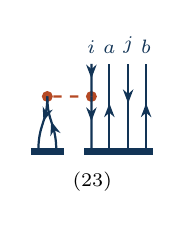
\begin{tikzpicture}[fcidiagram,baseline={(0,0)},scale=0.72]
    \draw[amp] (-0.40,0) -- (0.40,0);
    \draw[amp] (0.90,0) -- (2.60,0);
    \node[vtx] (h0) at (0.00,1.35) {}; \node[vtx] (h1) at (1.08,1.35) {}; \draw[vint] (h0) -- (h1);
    \draw[hline] (-0.22,0) .. controls (-0.22,0.7) and (0.00,0.7) .. (h0.center);
    \draw[pline] (0.22,0) .. controls (0.22,0.7) and (0.00,0.7) .. (h0.center);
    \draw[hline] (1.08,0) .. controls (1.08,0.7) and (1.08,0.7) .. (h1.center);
    \draw[hline] (h1.center) -- (1.08,2.15) node[dlab,above] {$i$};
    \draw[pline] (1.52,0) -- (1.52,2.15) node[dlab,above] {$a$};
    \draw[hline] (1.98,0) -- (1.98,2.15) node[dlab,above] {$j$};
    \draw[pline] (2.42,0) -- (2.42,2.15) node[dlab,above] {$b$};
    \node[dlab,below] at (1.10,-0.25) {(23)};
\end{tikzpicture} &
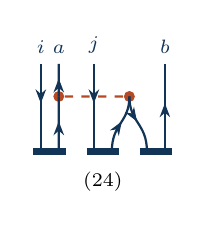
\begin{tikzpicture}[fcidiagram,baseline={(0,0)},scale=0.72]
    \draw[amp] (-0.40,0) -- (0.40,0);
    \draw[amp] (0.90,0) -- (1.70,0);
    \draw[amp] (2.20,0) -- (3.00,0);
    \node[vtx] (h0) at (0.22,1.35) {}; \node[vtx] (h1) at (1.95,1.35) {}; \draw[vint] (h0) -- (h1);
    \draw[pline] (h0.center) -- (0.22,2.15) node[dlab,above] {$a$};
    \draw[pline] (0.22,0) .. controls (0.22,0.7) and (0.22,0.7) .. (h0.center);
    \draw[hline] (2.38,0) .. controls (2.38,0.7) and (1.95,0.7) .. (h1.center);
    \draw[pline] (1.52,0) .. controls (1.52,0.7) and (1.95,0.7) .. (h1.center);
    \draw[hline] (-0.22,0) -- (-0.22,2.15) node[dlab,above] {$i$};
    \draw[hline] (1.08,0) -- (1.08,2.15) node[dlab,above] {$j$};
    \draw[pline] (2.82,0) -- (2.82,2.15) node[dlab,above] {$b$};
    \node[dlab,below] at (1.30,-0.25) {(24)};
\end{tikzpicture} &
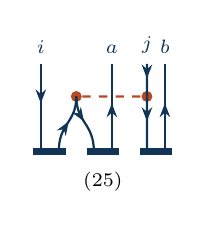
\begin{tikzpicture}[fcidiagram,baseline={(0,0)},scale=0.72]
    \draw[amp] (-0.40,0) -- (0.40,0);
    \draw[amp] (0.90,0) -- (1.70,0);
    \draw[amp] (2.20,0) -- (3.00,0);
    \node[vtx] (h0) at (0.65,1.35) {}; \node[vtx] (h1) at (2.38,1.35) {}; \draw[vint] (h0) -- (h1);
    \draw[hline] (1.08,0) .. controls (1.08,0.7) and (0.65,0.7) .. (h0.center);
    \draw[pline] (0.22,0) .. controls (0.22,0.7) and (0.65,0.7) .. (h0.center);
    \draw[hline] (2.38,0) .. controls (2.38,0.7) and (2.38,0.7) .. (h1.center);
    \draw[hline] (h1.center) -- (2.38,2.15) node[dlab,above] {$j$};
    \draw[hline] (-0.22,0) -- (-0.22,2.15) node[dlab,above] {$i$};
    \draw[pline] (1.52,0) -- (1.52,2.15) node[dlab,above] {$a$};
    \draw[pline] (2.82,0) -- (2.82,2.15) node[dlab,above] {$b$};
    \node[dlab,below] at (1.30,-0.25) {(25)};
\end{tikzpicture} &
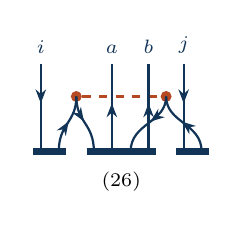
\begin{tikzpicture}[fcidiagram,baseline={(0,0)},scale=0.72]
    \draw[amp] (-0.40,0) -- (0.40,0);
    \draw[amp] (0.90,0) -- (2.60,0);
    \draw[amp] (3.10,0) -- (3.90,0);
    \node[vtx] (h0) at (0.65,1.35) {}; \node[vtx] (h1) at (2.85,1.35) {}; \draw[vint] (h0) -- (h1);
    \draw[hline] (1.08,0) .. controls (1.08,0.7) and (0.65,0.7) .. (h0.center);
    \draw[pline] (0.22,0) .. controls (0.22,0.7) and (0.65,0.7) .. (h0.center);
    \draw[hline] (1.98,0) .. controls (1.98,0.7) and (2.85,0.7) .. (h1.center);
    \draw[pline] (3.72,0) .. controls (3.72,0.7) and (2.85,0.7) .. (h1.center);
    \draw[hline] (-0.22,0) -- (-0.22,2.15) node[dlab,above] {$i$};
    \draw[pline] (1.52,0) -- (1.52,2.15) node[dlab,above] {$a$};
    \draw[pline] (2.42,0) -- (2.42,2.15) node[dlab,above] {$b$};
    \draw[hline] (3.28,0) -- (3.28,2.15) node[dlab,above] {$j$};
    \node[dlab,below] at (1.75,-0.25) {(26)};
\end{tikzpicture}
\end{tabular}

\vspace{0.35em}
\begin{tabular}{@{}c@{\hspace{1.6em}}c@{\hspace{1.6em}}c@{\hspace{1.6em}}c@{\hspace{1.6em}}c@{}}
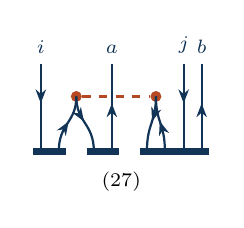
\begin{tikzpicture}[fcidiagram,baseline={(0,0)},scale=0.72]
    \draw[amp] (-0.40,0) -- (0.40,0);
    \draw[amp] (0.90,0) -- (1.70,0);
    \draw[amp] (2.20,0) -- (3.90,0);
    \node[vtx] (h0) at (0.65,1.35) {}; \node[vtx] (h1) at (2.60,1.35) {}; \draw[vint] (h0) -- (h1);
    \draw[hline] (1.08,0) .. controls (1.08,0.7) and (0.65,0.7) .. (h0.center);
    \draw[pline] (0.22,0) .. controls (0.22,0.7) and (0.65,0.7) .. (h0.center);
    \draw[hline] (2.38,0) .. controls (2.38,0.7) and (2.60,0.7) .. (h1.center);
    \draw[pline] (2.82,0) .. controls (2.82,0.7) and (2.60,0.7) .. (h1.center);
    \draw[hline] (-0.22,0) -- (-0.22,2.15) node[dlab,above] {$i$};
    \draw[pline] (1.52,0) -- (1.52,2.15) node[dlab,above] {$a$};
    \draw[hline] (3.28,0) -- (3.28,2.15) node[dlab,above] {$j$};
    \draw[pline] (3.72,0) -- (3.72,2.15) node[dlab,above] {$b$};
    \node[dlab,below] at (1.75,-0.25) {(27)};
\end{tikzpicture} &
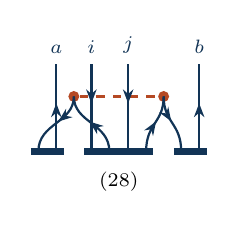
\begin{tikzpicture}[fcidiagram,baseline={(0,0)},scale=0.72]
    \draw[amp] (-0.40,0) -- (0.40,0);
    \draw[amp] (0.90,0) -- (2.60,0);
    \draw[amp] (3.10,0) -- (3.90,0);
    \node[vtx] (h0) at (0.65,1.35) {}; \node[vtx] (h1) at (2.85,1.35) {}; \draw[vint] (h0) -- (h1);
    \draw[hline] (-0.22,0) .. controls (-0.22,0.7) and (0.65,0.7) .. (h0.center);
    \draw[pline] (1.52,0) .. controls (1.52,0.7) and (0.65,0.7) .. (h0.center);
    \draw[hline] (3.28,0) .. controls (3.28,0.7) and (2.85,0.7) .. (h1.center);
    \draw[pline] (2.42,0) .. controls (2.42,0.7) and (2.85,0.7) .. (h1.center);
    \draw[pline] (0.22,0) -- (0.22,2.15) node[dlab,above] {$a$};
    \draw[hline] (1.08,0) -- (1.08,2.15) node[dlab,above] {$i$};
    \draw[hline] (1.98,0) -- (1.98,2.15) node[dlab,above] {$j$};
    \draw[pline] (3.72,0) -- (3.72,2.15) node[dlab,above] {$b$};
    \node[dlab,below] at (1.75,-0.25) {(28)};
\end{tikzpicture} &
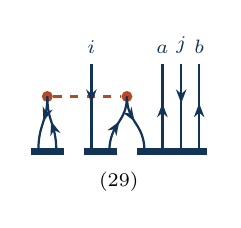
\begin{tikzpicture}[fcidiagram,baseline={(0,0)},scale=0.72]
    \draw[amp] (-0.40,0) -- (0.40,0);
    \draw[amp] (0.90,0) -- (1.70,0);
    \draw[amp] (2.20,0) -- (3.90,0);
    \node[vtx] (h0) at (0.00,1.35) {}; \node[vtx] (h1) at (1.95,1.35) {}; \draw[vint] (h0) -- (h1);
    \draw[hline] (-0.22,0) .. controls (-0.22,0.7) and (0.00,0.7) .. (h0.center);
    \draw[pline] (0.22,0) .. controls (0.22,0.7) and (0.00,0.7) .. (h0.center);
    \draw[hline] (2.38,0) .. controls (2.38,0.7) and (1.95,0.7) .. (h1.center);
    \draw[pline] (1.52,0) .. controls (1.52,0.7) and (1.95,0.7) .. (h1.center);
    \draw[hline] (1.08,0) -- (1.08,2.15) node[dlab,above] {$i$};
    \draw[pline] (2.82,0) -- (2.82,2.15) node[dlab,above] {$a$};
    \draw[hline] (3.28,0) -- (3.28,2.15) node[dlab,above] {$j$};
    \draw[pline] (3.72,0) -- (3.72,2.15) node[dlab,above] {$b$};
    \node[dlab,below] at (1.75,-0.25) {(29)};
\end{tikzpicture} &
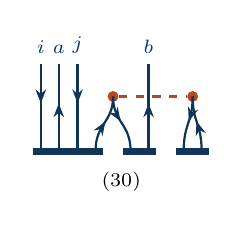
\begin{tikzpicture}[fcidiagram,baseline={(0,0)},scale=0.72]
    \draw[amp] (-0.40,0) -- (1.30,0);
    \draw[amp] (1.80,0) -- (2.60,0);
    \draw[amp] (3.10,0) -- (3.90,0);
    \node[vtx] (h0) at (1.55,1.35) {}; \node[vtx] (h1) at (3.50,1.35) {}; \draw[vint] (h0) -- (h1);
    \draw[hline] (1.98,0) .. controls (1.98,0.7) and (1.55,0.7) .. (h0.center);
    \draw[pline] (1.12,0) .. controls (1.12,0.7) and (1.55,0.7) .. (h0.center);
    \draw[hline] (3.28,0) .. controls (3.28,0.7) and (3.50,0.7) .. (h1.center);
    \draw[pline] (3.72,0) .. controls (3.72,0.7) and (3.50,0.7) .. (h1.center);
    \draw[hline] (-0.22,0) -- (-0.22,2.15) node[dlab,above] {$i$};
    \draw[pline] (0.22,0) -- (0.22,2.15) node[dlab,above] {$a$};
    \draw[hline] (0.68,0) -- (0.68,2.15) node[dlab,above] {$j$};
    \draw[pline] (2.42,0) -- (2.42,2.15) node[dlab,above] {$b$};
    \node[dlab,below] at (1.75,-0.25) {(30)};
\end{tikzpicture} &
\begin{tikzpicture}[fcidiagram,baseline={(0,0)},scale=0.72]
    \draw[amp] (-0.40,0) -- (0.40,0);
    \draw[amp] (0.90,0) -- (1.70,0);
    \draw[amp] (2.20,0) -- (3.00,0);
    \draw[amp] (3.50,0) -- (4.30,0);
    \node[vtx] (h0) at (0.65,1.35) {}; \node[vtx] (h1) at (3.25,1.35) {}; \draw[vint] (h0) -- (h1);
    \draw[hline] (1.08,0) .. controls (1.08,0.7) and (0.65,0.7) .. (h0.center);
    \draw[pline] (0.22,0) .. controls (0.22,0.7) and (0.65,0.7) .. (h0.center);
    \draw[hline] (3.68,0) .. controls (3.68,0.7) and (3.25,0.7) .. (h1.center);
    \draw[pline] (2.82,0) .. controls (2.82,0.7) and (3.25,0.7) .. (h1.center);
    \draw[hline] (-0.22,0) -- (-0.22,2.15) node[dlab,above] {$i$};
    \draw[pline] (1.52,0) -- (1.52,2.15) node[dlab,above] {$a$};
    \draw[hline] (2.38,0) -- (2.38,2.15) node[dlab,above] {$j$};
    \draw[pline] (4.12,0) -- (4.12,2.15) node[dlab,above] {$b$};
    \node[dlab,below] at (1.95,-0.25) {(31)};
\end{tikzpicture}
\end{tabular}
\end{center}
\footnotesize
(17)--(23) $T_1T_2$; (24), (25) three $T_1$; (26)--(30) $T_1^2T_2$; (31) four $T_1$ on $\as mnef$: the quartic term, and the four-cluster limit of the Baker-Campbell-Hausdorff series realised. Every one of these fifteen is a CCD diagram with $T_1$ bars hung on the lines of its $H_N$ fragment.
\end{frame}

\begin{frame}{The doubles equation, read off}
\scriptsize
\begin{align*}
0={}&\as abij+P(ij)\as abej\,t_i^e-P(ab)\as amij\,t_m^b+P(ab)f_{be}t_{ij}^{ae}-P(ij)f_{mi}t_{mj}^{ab}
 +\tfrac12\as abef\,t_{ij}^{ef}+\tfrac12\as mnij\,t_{mn}^{ab}\\
 &+P(ij)P(ab)\as mbej\,t_{im}^{ae}
 +\tfrac12P(ij)\as abef\,t_i^et_j^f+\tfrac12P(ab)\as mnij\,t_m^at_n^b-P(ij)P(ab)\as mbej\,t_i^et_m^a\\
 &+\tfrac14\as mnef\,t_{ij}^{ef}t_{mn}^{ab}+\tfrac12P(ij)P(ab)\as mnef\,t_{im}^{ae}t_{nj}^{fb}
 -\tfrac12P(ab)\as mnef\,t_{ij}^{ae}t_{mn}^{bf}-\tfrac12P(ij)\as mnef\,t_{mi}^{ef}t_{nj}^{ab}\\
 &-P(ij)f_{me}t_i^et_{mj}^{ab}-P(ab)f_{me}t_{ij}^{ae}t_m^b
 +P(ij)P(ab)\as amef\,t_i^et_{mj}^{fb}-\tfrac12P(ab)\as amef\,t_{ij}^{ef}t_m^b+P(ab)\as bmef\,t_{ij}^{ae}t_m^f\\
 &-P(ij)P(ab)\as mnej\,t_{im}^{ae}t_n^b+\tfrac12P(ij)\as mnej\,t_i^et_{mn}^{ab}-P(ij)\as mnei\,t_m^et_{nj}^{ab}\\
 &-\tfrac12P(ij)P(ab)\as amef\,t_i^et_j^ft_m^b+\tfrac12P(ij)P(ab)\as mnej\,t_i^et_m^at_n^b
 +\tfrac14P(ij)\as mnef\,t_i^et_{mn}^{ab}t_j^f-P(ij)P(ab)\as mnef\,t_i^et_m^at_{nj}^{fb}\\
 &+\tfrac14P(ab)\as mnef\,t_m^at_{ij}^{ef}t_n^b-P(ij)\as mnef\,t_m^et_i^ft_{nj}^{ab}-P(ab)\as mnef\,t_{ij}^{ae}t_m^bt_n^f
 +\tfrac14P(ij)P(ab)\as mnef\,t_i^et_m^at_j^ft_n^b
\end{align*}
\small
\begin{itemize}
\item Thirty-one terms in the order of the diagrams: (1), (4)--(8) linear; (2), (3) linear in $t_1$; (9)--(23) quadratic; (24)--(30) cubic; (31) quartic.
\item Nobody programs this line by line. But every term can be seen, counted and checked: all signs agree with $(-1)^{h+l}$ evaluated by a twenty-line script, and the sum agrees with $e^{-T}He^{T}$ in determinant space (\texttt{ccsd\_diagrams.py}, \texttt{week48.ipynb}).
\end{itemize}
\end{frame}

\begin{frame}{Pause to think \#2}
\thinkq{4}{\normalsize
\begin{columns}[c]
\column{0.3\textwidth}
\centering
\begin{tikzpicture}[fcidiagram,dlab/.style={font=\small},scale=1.9]
    \draw[amp] (-0.40,0) -- (0.40,0);
    \draw[amp] (0.90,0) -- (1.70,0);
    \node[vtx] (h0) at (0.65,1.35) {}; \node[vtx] (h1) at (2.45,1.35) {}; \draw[vint] (h0) -- (h1);
    \draw[hline] (1.08,0) .. controls (1.08,0.7) and (0.65,0.7) .. (h0.center);
    \draw[pline] (0.22,0) .. controls (0.22,0.7) and (0.65,0.7) .. (h0.center);
    \draw[pline] (h1.center) -- (2.78,2.15) node[dlab,above] {$b$};
    \draw[hline] (h1.center) -- (2.12,2.15) node[dlab,above] {$j$};
    \draw[hline] (-0.22,0) -- (-0.22,2.15) node[dlab,above] {$i$};
    \draw[pline] (1.52,0) -- (1.52,2.15) node[dlab,above] {$a$};
    \node[dlab,below] at (0.65,-0.25) {(11)};
\end{tikzpicture}
\column{0.7\textwidth}
Diagram (11) of the doubles equation.
\begin{enumerate}
\item Read it: matrix element, amplitudes, sign, factors, permutations.
\item Which diagram of CCD is it a relative of, and how?
\item Which term of the \emph{dressed} equation of lecture 1 contains it? Why does it come with a minus sign there, without any counting of loops?
\end{enumerate}
\end{columns}}
\end{frame}

\begin{frame}[shrink=1]{Answer to pause \#2}
\thinka{%
\begin{enumerate}
\item A particle line $e$ from one single and a hole line $m$ from another enter the left vertex of $\as mbej$; the right vertex emits $(b,j)$. Hole lines $i,j,m$: $h=3$. Loops: $i\to e\to m\to a$ through the bra, and $(j,b)$: $l=2$. Sign $-$. No equivalent lines; the two singles are attached differently (one by its particle, one by its hole), so no $\tfrac12$. External lines from different operators: $P(ij)P(ab)$.
\[
 -P(ij)P(ab)\sum_{me}\as mbej\,t_i^e\,t_m^a
\]
\item The ring, diagram (8), $+P(ij)P(ab)\as mbej t_{im}^{ae}$, with the $T_2$ bar cut into two $T_1$ bars. The loop $(m,e)$ of the ring is opened: one loop fewer, opposite sign.
\item The dressed driving term $\vt abij$: dress $a\to-t_m^a(m)$ on a creator and $i\to+t_i^e(e)$ on an annihilator of $\as abij$, giving $-\as mbej t_m^at_i^e$. The minus sign is the one in $X=1-t_1$.
\end{enumerate}}
\end{frame}

\begin{frame}[shrink=13]{From diagrams to intermediates}
\footnotesize
Programs do not dress integrals index by index either; they collect diagrams that share a bar attached in the same way. The standard set (Stanton, Gauss, Watts and Bartlett 1991), with $\tilde\tau_{ij}^{ab}=t_{ij}^{ab}+\tfrac12(t_i^at_j^b-t_i^bt_j^a)$:
\begin{align*}
F_{ae}&=f'_{ae}-\tfrac12f_{me}t_m^a+t_m^f\as mafe-\tfrac12\tilde\tau_{mn}^{af}\as mnef,&
F_{mi}&=f'_{mi}+\tfrac12t_i^ef_{me}+t_n^e\as mnie+\tfrac12\tilde\tau_{in}^{ef}\as mnef,\\
F_{me}&=f_{me}+t_n^f\as mnef,&
W_{mnij}&=\as mnij+P(ij)t_j^e\as mnie+\tfrac14\tau_{ij}^{ef}\as mnef,\\
W_{abef}&=\as abef-P(ab)t_m^b\as amef+\tfrac14\tau_{mn}^{ab}\as mnef,&
W_{mbej}&=\as mbej+t_j^f\as mbef-t_n^b\as mnej\\
&&&\quad-(\tfrac12t_{jn}^{fb}+t_j^ft_n^b)\as mnef .
\end{align*}
\begin{align*}
D_i^at_i^a={}&f_{ia}+t_i^eF_{ae}-t_m^aF_{mi}+t_{im}^{ae}F_{me}-t_n^f\as naif-\tfrac12t_{im}^{ef}\as maef-\tfrac12t_{mn}^{ae}\as nmei,\\
D_{ij}^{ab}t_{ij}^{ab}={}&\as ijab+P(ab)t_{ij}^{ae}\bigl(F_{be}-\tfrac12t_m^bF_{me}\bigr)-P(ij)t_{im}^{ab}\bigl(F_{mj}+\tfrac12t_j^eF_{me}\bigr)
 +\tfrac12\tau_{mn}^{ab}W_{mnij}+\tfrac12\tau_{ij}^{ef}W_{abef}\\
 &+P(ij)P(ab)\bigl(t_{im}^{ae}W_{mbej}-t_i^et_m^a\as mbej\bigr)+P(ij)t_i^e\as abej-P(ab)t_m^a\as mbij .
\end{align*}
\small
\begin{itemize}
\item Each intermediate is a bare integral plus corrections in which amplitudes dress it: $F$ the Fock matrix, $W_{mnij}$, $W_{abef}$ the ladders, $W_{mbej}$ the ring. $F_{me}$ is the $\ft_{kc}$ of lecture 1.
\item Never form an object with more indices than the answer has: every contraction is at most $n^6$. This is \texttt{coupledcluster.py}, and every production code.
\item Different factorisations are different groupings of the same $14+31$ diagrams. All give the same numbers (checked).
\end{itemize}
\end{frame}

\begin{frame}[shrink=16]{When singles matter}
\small
\begin{columns}[T]
\column{0.5\textwidth}
The pairing model with a term that breaks pairs (chapter 10, section 10.10):
\[
 V_{\rm ph}=-\frac f2\sum_{pqr}\bigl(\cre{p+}\cre{p-}\ann{q-}\ann{r+}+\text{h.c.}\bigr)
\]
\begin{center}
\scriptsize\setlength{\tabcolsep}{3pt}\renewcommand{\arraystretch}{1.15}
\begin{tabular}{rrrrrr}
\toprule
$g$ & $f$ & CCD & CCSD & exact & $\max|t_1|$\\
\midrule
0.50 & 0.000 & 1.41664 & 1.41664 & 1.41677 & 0\\
0.50 & 0.025 & 1.34760 & 1.34691 & 1.34713 & 0.011\\
0.70 & 0.050 & 0.97076 & 0.96815 & 0.96976 & 0.019\\
1.00 & 0.050 & 0.44474 & 0.44237 & 0.45058 & 0.017\\
0.50 & 0.250 & 0.60331 & 0.54672 & 0.55119 & 0.084\\
\bottomrule
\end{tabular}
\end{center}
Four levels, four particles, bare reference. At $g=0.5$, $f=0.25$ the singles turn a nine per cent error in the energy into one below one per cent.
\column{0.5\textwidth}
\centering
\tikzset{every picture/.style={scale=1}}\begin{tikzpicture}[scale=1]
\begin{axis}[width=6.6cm,height=4.9cm,xlabel={$f$ \ ($g=0.5$)},ylabel={energy},xmin=0,xmax=0.5,grid=major,legend style={font=\scriptsize,at={(.03,.03)},anchor=south west},tick label style={font=\scriptsize},label style={font=\small}]
\addplot[black,only marks,mark=*,mark size=1.3pt] coordinates {(0.00,1.41677) (0.05,1.27347) (0.10,1.11435) (0.15,0.94020) (0.20,0.75208) (0.25,0.55119) (0.30,0.33879) (0.35,0.11614) (0.40,-0.11558) (0.45,-0.35529) (0.50,-0.60204)};\addlegendentry{exact}
\addplot[blue,thick] coordinates {(0.00,1.41664) (0.05,1.27585) (0.10,1.12413) (0.15,0.96142) (0.20,0.78776) (0.25,0.60331) (0.30,0.40833) (0.35,0.20313) (0.40,-0.01194) (0.45,-0.23647) (0.50,-0.47008)};\addlegendentry{CCD}
\addplot[red,thick] coordinates {(0.00,1.41664) (0.05,1.27311) (0.10,1.11357) (0.15,0.93868) (0.20,0.74938) (0.25,0.54672) (0.30,0.33183) (0.35,0.10583) (0.40,-0.13023) (0.45,-0.37541) (0.50,-0.62885)};\addlegendentry{CCSD}
\end{axis}
\end{tikzpicture}

\raggedright\footnotesize The largest singles amplitude grows linearly from zero ($0.021$ at $f=0.05$, $0.128$ at $f=0.5$): on the bare reference $f_{ai}\ne0$ and the singles are of first order.
\end{columns}
\begin{itemize}
\item $f=0$: seniority is conserved, $T_1=0$ identically, CCSD $=$ CCD. Nothing about the doubles changes with $f$; the Hamiltonian acquires a channel the doubles cannot reach.
\item On the Hartree-Fock reference the singles are an order of magnitude smaller (Brillouin) and the CCSD energies nearly the same: $1.3469088$ against $1.3469075$ at $g=0.5$, $f=0.025$. Truncated coupled cluster depends on the reference -- weakly, thanks to $T_1$.
\end{itemize}
\end{frame}

\begin{frame}[shrink=16]{Beyond CCSD}
\small
\begin{columns}[T]
\column{0.5\textwidth}
\begin{block}{Up the hierarchy}
\begin{itemize}
\item CCSDT: $T_3$ and a triples equation $0=\mel{\Phi_{ijk}^{abc}}{\Hbar_N}{\ph}$; cost $n^8$.
\item CCSD(T): triples from the converged $t_1,t_2$ by perturbation theory; no iteration, cost $n^7$, correct through fourth order. The ``gold standard'' of quantum chemistry.
\item For the pairing model the missing cluster is $T_4$, not $T_3$ (week 47).
\end{itemize}
\end{block}
\begin{block}{Excited states and properties}
$\Hbar_N$ is not Hermitian: left and right eigenvectors differ, and expectation values need both ($\Lambda$ equations). Diagonalising $\Hbar_N$ among singles and doubles gives excitation energies: equation-of-motion coupled cluster.
\end{block}
\column{0.5\textwidth}
\begin{block}{Other exponentials}
\begin{itemize}
\item Unitary coupled cluster, $e^{T-T^\dagger}$: a variational energy, a series that does not terminate; the natural ansatz for a quantum computer (chapter 10, sections 10.15--10.16; FYS5419).
\item In-medium SRG: a continuous unitary transformation that decouples the reference, solved as a flow equation.
\end{itemize}
\end{block}
\begin{block}{Where single-reference coupled cluster ends}
Strong static correlation: bond breaking, strong pairing, open-shell nuclei. There the reference itself must change: symmetry breaking, multi-reference methods, or the tensor networks of weeks 40--41.
\end{block}
\end{columns}
\vspace{0.4em}
What made coupled cluster the standard: size extensive by construction, systematically improvable by raising the rank of $T$, polynomial cost at fixed rank. No other method of this course has all three.
\end{frame}

\begin{frame}{Summary of Thursday}
\begin{itemize}
\item CCSD: $T=T_1+T_2$, three energy diagrams, fourteen for the singles, thirty-one for the doubles; at most four cluster operators on one vertex.
\item $e^{T_1}$ is an orbital transformation. $e^{-T_1}He^{T_1}$ is a one- plus two-body operator with dressed integrals $\tilde h=XhY^{T}$, $\tilde v=XXvY^{T}Y^{T}$, and
\[
 \Hbar=e^{-T_2}\tilde He^{T_2}:\quad\text{CCSD}=\text{CCD with }\tilde H\ +\ \text{a four-term singles equation}.
\]
\item With $T_2=0$ the singles equation is Hartree-Fock; with $T_1=0$ the doubles equation is CCD. In a Hartree-Fock basis the singles start at second order.
\item The $14+31$ diagrams sort into families, one per dressed vertex. Intermediates are the same families collected for efficient evaluation; the cost stays $n^6$.
\item Singles matter when the interaction, or the reference, couples the reference to single excitations. They make the result nearly independent of the orbitals.
\item Beyond: triples (CCSD(T)), excited states (EOM), unitary and in-medium variants.
\end{itemize}
\end{frame}

% ======================================================================
\section[Friday 3: Review, part 1]{Friday, lecture 3: The semester in review, part 1}
% ======================================================================

\begin{frame}[shrink=13]{One sentence, fourteen weeks}
\begin{exampleblock}{The sentence from the first lecture (week 34)}
The many-body problem is linear algebra in a space that is exponentially large; every method we study is a strategy for not having to look at all of it.
\end{exampleblock}
\small
\begin{center}
\renewcommand{\arraystretch}{1.12}
\begin{tabular}{lll}
\toprule
weeks & topic & lecture notes\\
\midrule
34 & many-body wave functions, notation, linear algebra & chapters 1--2\\
35--37 & second quantization, Wick's theorem, particle-hole formalism & chapter 3\\
38 & full configuration interaction, truncations, size consistency & chapter 5\\
39 & Hartree-Fock theory, Thouless' theorem, stability & chapter 6\\
40--41 & matrix product states, matrix product operators, DMRG & chapter 11\\
42--43 & the electron gas; density functional theory & chapters 6 and 8\\
44 & many-body perturbation theory & chapter 9\\
45--46 & diagram rules, third order, the linked-diagram theorem & chapter 9\\
46--48 & coupled-cluster theory: CCD and CCSD & chapter 10\\
\bottomrule
\end{tabular}
\end{center}
Two midterms on one model, the pairing Hamiltonian: exact diagonalisation, Hartree-Fock and DMRG in the first; perturbation theory and its diagrams in the second; coupled cluster in the lectures of the last two weeks.
\end{frame}

\begin{frame}[shrink=22]{Second quantization: the language (weeks 34--37)}
\small
\begin{columns}[T]
\column{0.52\textwidth}
\begin{block}{What it is}
\[
 \{\ann p,\cre q\}=\delta_{pq},\qquad\{\ann p,\ann q\}=\{\cre p,\cre q\}=0,
\]
\[
 H=\sum_{pq}h_{pq}\cre p\ann q+\tfrac14\!\sum_{pqrs}\!\as pqrs\cre p\cre q\ann s\ann r .
\]
Antisymmetry is carried by the operators, not by the bookkeeping of determinants. One formula for every particle number.
\end{block}
\begin{block}{Wick's theorem}
A product of operators is its normal-ordered form plus all contractions. Relative to a reference $\ket{\ph}$: $\ann a\cre b\to\delta_{ab}$, $\cre i\ann j\to\delta_{ij}$. Expectation values in $\ket{\ph}$ are sums of full contractions.
\end{block}
\column{0.48\textwidth}
\begin{block}{The normal-ordered Hamiltonian}
\begin{align*}
 H&=\Eref+\sum_{pq}f_{pq}\no{\cre p\ann q}\\
 &\quad+\tfrac14\sum_{pqrs}\as pqrs\no{\cre p\cre q\ann s\ann r},\\
 \Eref&=\sum_ih_{ii}+\tfrac12\sum_{ij}\as ijij,\quad f_{pq}=h_{pq}+\sum_i\as piqi .
\end{align*}
The mean field has been summed once and for all; what remains acts on particles and holes.
\end{block}
\begin{block}{You should be able to}
\begin{itemize}
\item derive the Condon-Slater rules with Wick's theorem;
\item normal-order $H$ relative to a determinant;
\item evaluate $\mel{\Phi_i^a}{H}{\Phi_j^b}$ and friends;
\item explain the generalised theorem and why it makes everything after week 37 possible.
\end{itemize}
\end{block}
\end{columns}
\end{frame}

\begin{frame}[shrink=1]{Full configuration interaction: the exact answer (week 38)}
\small
\begin{columns}[T]
\column{0.5\textwidth}
\begin{block}{The method}
Expand in all determinants, $\ket{\Psi}=\sum_IC_I\ket{\Phi_I}$, and diagonalise:
\[
 \sum_J\mel{\Phi_I}{H}{\Phi_J}C_J=E\,C_I .
\]
The Rayleigh-Ritz variational principle: $E_0$ is an upper bound that improves monotonically with the basis (Hylleraas-Undheim-MacDonald).
\end{block}
\begin{block}{The wall}
$\binom{n}{N}$ determinants: $70$ for the pairing model with four levels and four particles ($6$ without broken pairs), $3.5\times10^{10}$ for $19$ particles in $38$ orbitals.
\end{block}
\column{0.5\textwidth}
\begin{block}{Truncations and their defect}
$\ket{\Psi}=(1+C_1+C_2+\cdots)\ket{\ph}$ cut at doubles (CISD) is variational but \alert{not size consistent}: two non-interacting systems are not described as well as each one separately, because the product $C_2^AC_2^B$ is a quadruple.
\end{block}
\begin{block}{You should be able to}
\begin{itemize}
\item set up the Hamiltonian matrix in a particle-hole basis and say which blocks vanish;
\item derive the eigenvalue problem from the variational principle;
\item write the projected equations for $C_1$, $C_2$ and draw them;
\item explain size consistency with two copies.
\end{itemize}
\end{block}
\end{columns}
\vspace{0.3em}
FCI is the benchmark for everything else: every table of this course has it in the last column.
\end{frame}

\begin{frame}[shrink=7]{Hartree-Fock: the best single determinant (week 39)}
\small
\begin{columns}[T]
\column{0.5\textwidth}
\begin{block}{The method}
Minimise $\mel{\Phi}{H}{\Phi}$ over all Slater determinants. The stationarity condition is
\[
 f_{ai}=\mel{a}{h}{i}+\sum_j\as ajij=0\qquad\text{(Brillouin)},
\]
solved self-consistently as $f\,\phi_p=\varepsilon_p\phi_p$.
\[
 E_{\rm HF}=\sum_i\varepsilon_i-\tfrac12\sum_{ij}\as ijij .
\]
\end{block}
\begin{block}{Thouless' theorem}
Any determinant not orthogonal to $\ket{\ph}$ is $e^{T_1}\ket{\ph}$ (up to normalisation). Yesterday: this is the $T_1$ of coupled cluster.
\end{block}
\column{0.5\textwidth}
\begin{block}{Stability}
Stationary is not minimal. The second variation gives the matrix
$\begin{pmatrix}A&B\\B^*&A^*\end{pmatrix}$ -- the RPA matrix. A negative eigenvalue: a lower determinant exists, usually with a broken symmetry (Lipkin model beyond $\chi=1$).
\end{block}
\begin{block}{You should be able to}
\begin{itemize}
\item derive the Hartree-Fock equations by varying the coefficients, and in second quantization by varying one orbital;
\item state and use Brillouin's and Koopmans' theorems;
\item explain why Hartree-Fock ``does nothing'' for the pairing model ($E=2-g$) and what that says about correlation.
\end{itemize}
\end{block}
\end{columns}
\end{frame}

\begin{frame}[shrink=4]{Matrix product states and the DMRG (weeks 40--41)}
\small
\begin{columns}[T]
\column{0.5\textwidth}
\begin{block}{The idea}
Truncate not by excitation rank but by \emph{entanglement}. Cut the system in two; the Schmidt decomposition
\[
 \ket{\Psi}=\sum_{\alpha=1}^{\chi}s_\alpha\ket{\alpha}_L\ket{\alpha}_R
\]
is the best approximation of rank $\chi$. Repeated at every cut: a matrix product state, $d\,L\,\chi^2$ numbers instead of $d^L$.
\end{block}
\begin{block}{The algorithm}
The Hamiltonian as a matrix product operator; sweep through the sites, solving a small eigenvalue problem for one or two tensors at a time; cost $\propto L\chi^3$. Variational: the energy is an upper bound.
\end{block}
\column{0.5\textwidth}
\begin{block}{Where it wins, where it does not}
Ground states of gapped one-dimensional Hamiltonians obey an area law: small $\chi$ suffices and the DMRG is practically exact (Heisenberg chain, $L=32$: twelve digits). In higher dimensions, or with long-range entanglement, $\chi$ grows quickly.
\end{block}
\begin{block}{You should be able to}
\begin{itemize}
\item explain the Schmidt decomposition and the discarded weight;
\item write a simple Hamiltonian as an MPO;
\item describe one sweep and the convergence checks;
\item compare the DMRG results of the first midterm for the pairing model with FCI.
\end{itemize}
\end{block}
\end{columns}
\end{frame}

\begin{frame}[shrink=7]{The electron gas and density functional theory (weeks 42--43)}
\small
\begin{columns}[T]
\column{0.5\textwidth}
\begin{block}{The electron gas in Hartree-Fock}
Plane waves solve the Hartree-Fock equations by momentum conservation. Per particle, in Rydberg,
\[
 \frac EN=\frac{2.21}{r_s^2}-\frac{0.916}{r_s}:
\]
exchange alone binds the gas (minimum near $r_s=4.8$), but the single-particle spectrum is pathological at the Fermi surface. Correlation -- screening -- is essential.
\end{block}
\begin{block}{Hohenberg-Kohn}
The ground-state density determines the external potential, and the energy is a functional $E[n]$ minimised by the true density. Exact, and silent about what the functional is.
\end{block}
\column{0.5\textwidth}
\begin{block}{Kohn-Sham}
A non-interacting system with the same density:
\[
 \bigl(-\tfrac12\nabla^2+v_{\rm ext}+v_{\rm H}[n]+v_{\rm xc}[n]\bigr)\phi_i=\varepsilon_i\phi_i,
\]
with all the difficulty moved into $E_{\rm xc}[n]$. The local density approximation takes it from the electron gas, $\epsilon_x\propto-n^{1/3}$.
\end{block}
\begin{block}{You should be able to}
\begin{itemize}
\item derive the Hartree-Fock energy of the gas and discuss its defects;
\item prove the first Hohenberg-Kohn theorem;
\item compare Kohn-Sham with Hartree-Fock: what the orbitals and eigenvalues mean, self-interaction, why the result is not variational with an approximate functional.
\end{itemize}
\end{block}
\end{columns}
\end{frame}

% ======================================================================
\section[Friday 4: Review, part 2; the exam]{Friday, lecture 4: The semester in review, part 2, and the exam}
% ======================================================================

\begin{frame}[shrink=10]{Many-body perturbation theory (week 44)}
\small
\begin{columns}[T]
\column{0.5\textwidth}
\begin{block}{The method}
$H=H_0+H_I$, $P=\ket{\ph}\bra{\ph}$, $Q=1-P$, intermediate normalisation. One exact equation,
\[
 \ket{\Psi_0}=\ket{\ph}+\tfrac{Q}{\omega-H_0}\bigl(\omega-E_0+H_I\bigr)\ket{\Psi_0},
\]
and two choices of $\omega$: $\omega=E_0$ (Brillouin-Wigner) and $\omega=\varepsilon_0$ (Rayleigh-Schr\"odinger).
\[
 E^{(2)}=\sum_{m\ne0}\frac{|\mel{\Phi_m}{H_I}{\ph}|^2}{\varepsilon_0-\varepsilon_m}
 \overset{\rm HF}{=}\frac14\sum_{ijab}\frac{|\as abij|^2}{D_{ij}^{ab}}
\]
\end{block}
\column{0.5\textwidth}
\begin{block}{What to remember}
\begin{itemize}
\item Rayleigh-Schr\"odinger theory has renormalisation (folded) terms from third order on; Brillouin-Wigner has none, at the price of the unknown energy in every denominator.
\item Not variational. Convergence depends on the partition and on the coupling: for the pairing model the series is useful for $g\lesssim1$ and worthless beyond.
\item With a Hartree-Fock reference the singles do not contribute at second and third order.
\end{itemize}
\end{block}
\begin{block}{You should be able to}
derive the expansion from the projection operators; write $E^{(2)}$ and $E^{(3)}$; show that $Q/(\omega-H_0)$ is diagonal; compare the two schemes on a two-level model. (The second midterm.)
\end{block}
\end{columns}
\end{frame}

\begin{frame}[shrink=7]{Diagrams and the linked-diagram theorem (weeks 45--46)}
\small
\begin{columns}[T]
\column{0.5\textwidth}
\begin{block}{The rules are theorems}
A diagram is a class of equal Wick contraction patterns. Lines are contractions; a cut between vertices is a denominator $\sum\varepsilon_{\rm holes}-\sum\varepsilon_{\rm particles}$; the sign is $(-1)^{h+l}$; equivalent lines give $\tfrac12$.

Third order: fourteen diagrams, three without crosses -- the particle-particle ladder, the hole-hole ladder and the ring. Pairing model: $E^{(2)}=-\tfrac7{24}g^2$, $E^{(3)}=-\tfrac1{12}g^3$.
\end{block}
\begin{block}{Connected, linked, unlinked}
Unlinked diagrams have a closed piece detached from the rest. They scale with the wrong power of the particle number.
\end{block}
\column{0.5\textwidth}
\begin{block}{The theorem (Goldstone 1957)}
\[
 \Delta E=\sum_{n}\mel{\ph}{H_I\Bigl(\frac{Q}{\varepsilon_0-H_0}H_I\Bigr)^{n}}{\ph}_{\rm connected}
\]
The renormalisation terms cancel the unlinked diagrams, order by order, through the factorisation of denominators. Consequence: the energy of independent systems is additive at every order -- size extensivity.
\end{block}
\begin{block}{You should be able to}
\begin{itemize}
\item draw and evaluate all diagrams to third order;
\item explain the fourth-order cancellation with the two time orderings;
\item say what an exclusion-principle-violating diagram is and why it must be kept.
\end{itemize}
\end{block}
\end{columns}
\end{frame}

\begin{frame}[shrink=7]{Coupled-cluster theory (weeks 46--48)}
\small
\begin{columns}[T]
\column{0.5\textwidth}
\begin{block}{The method}
\[
 \ket{\Psi}=e^{T}\ket{\ph},\qquad \Hbar=e^{-T}He^{T}=\Eref+\bigl(H_Ne^{T}\bigr)_c,
\]
\[
 \Delta E=\av{\Hbar_N},\qquad 0=\mel{\Phi_\mu}{\Hbar_N}{\ph}.
\]
The linked-diagram theorem turned into an ansatz: the exponential generates all disconnected products of connected clusters, and the equations contain only connected terms.
\end{block}
\begin{block}{CCD and CCSD}
CCD: ten terms -- driving, Fock, two ladders, ring, four quadratic. CCSD: the same with a $T_1$-dressed Hamiltonian plus a singles equation; $3+14+31$ diagrams. Cost $n^6$.
\end{block}
\column{0.5\textwidth}
\begin{block}{What to remember}
\begin{itemize}
\item Size extensive at every truncation; exact for independent pairs (CCD).
\item Not variational: the energy is a projection, not an expectation value; it can lie below the exact one (pairing model, every $g$).
\item Sums ladders, rings and their couplings to all orders; correct through third order, with triples through fourth.
\item Fails where a single reference fails.
\end{itemize}
\end{block}
\begin{block}{You should be able to}
explain why the Baker-Campbell-Hausdorff series terminates; derive the CCD equation, analytically or with diagrams; reduce it for the pairing model; compare CCD with CID and with perturbation theory.
\end{block}
\end{columns}
\end{frame}

\begin{frame}{One model, every method: the pairing Hamiltonian}
\small
Four doubly degenerate levels, four particles, $\xi=1$; total ground-state energies.
\begin{center}
\setlength{\tabcolsep}{5pt}\renewcommand{\arraystretch}{1.15}
\begin{tabular}{@{}rrrrrrrr@{}}
\toprule
$g$ & HF & MBPT2 & MBPT3 & CID & HF+RPA & CCD & FCI\\
\midrule
0.25 & 1.75000 & 1.73177 & 1.73047 & 1.73051 & 1.71635 & 1.73046 & 1.73046\\
0.50 & 1.50000 & 1.42708 & 1.41667 & 1.41760 & 1.37450 & 1.41664 & 1.41677\\
1.00 & 1.00000 & 0.70833 & 0.62500 & 0.64891 & 0.55459 & 0.63044 & 0.63555\\
1.50 & 0.50000 & $-0.15625$ & $-0.43750$ & $-0.29113$ & $-0.40625$ & $-0.38417$ & $-0.34819$\\
2.00 & 0.00000 & $-1.16667$ & $-1.83333$ & $-1.35209$ & $-1.47622$ & $-1.60959$ & $-1.48965$\\
\bottomrule
\end{tabular}
\end{center}
\begin{itemize}
\item HF: $2-g$, no correlation at all. MBPT (bare one-body partition): $2-g-\tfrac7{24}g^2-\tfrac1{12}g^3$, excellent at $g=0.25$, lost at $g=2$. CID: always above FCI. CCD: closest at four of the five couplings, always below. DMRG (first midterm) reproduces the FCI column.
\item Upper bounds: HF, CID, DMRG, FCI. No bound: MBPT, RPA, CCD.
\item The table is a comparison for this model, not a ranking. At $g=2$ the RPA happens to be closest; with five pairs CCD deteriorates sooner (week 47).
\end{itemize}
\end{frame}

\begin{frame}[shrink=10]{How the methods relate}
\small
\begin{center}
\renewcommand{\arraystretch}{1.25}
\begin{tabular}{llllll}
\toprule
method & what is truncated & upper bound & size extensive & improvable & cost\\
\midrule
Hartree-Fock & everything but one determinant & yes & yes & no & $n^4$\\
CISD & excitation rank of $C$ & yes & \alert{no} & yes ($\to$ FCI) & $n^6$\\
FCI & nothing & yes & yes & exact & $\binom nN$\\
DMRG & entanglement ($\chi$) & yes & yes & yes ($\chi\to\infty$) & $L\chi^3$\\
MBPT($k$) & order in $H_I$ & no & yes & may diverge & $n^5$, $n^6$, \dots\\
RPA & ring diagrams only & no & yes & no & $n^6$\\
CCSD & excitation rank of $T$ & no & yes & yes ($\to$ FCI) & $n^6$\\
Kohn-Sham DFT & the functional & no & yes & not systematically & $n^3$\\
\bottomrule
\end{tabular}
\end{center}
\begin{itemize}
\item Truncating the \emph{linear} expansion (CI) keeps the bound and loses extensivity; truncating the \emph{exponential} (CC) or the \emph{order} (MBPT) keeps extensivity and loses the bound. Only untruncated methods have both.
\item The same objects recur: the first-order doubles amplitude is the MP2 wave function, the first CC iteration and the first CI correction; the stability matrix of Hartree-Fock is the RPA matrix; Thouless' $e^{T_1}$ is the singles of CCSD; the unlinked diagrams of MBPT are the $-\Delta E\,C$ of CI.
\end{itemize}
\end{frame}

\begin{frame}{Pause to think \#3}
\thinkq{5}{\normalsize True or false -- and why? (Oral-exam warm-up.)
\begin{enumerate}
\item The Hartree-Fock energy is an upper bound to the exact ground-state energy.
\item The second-order energy of the ground state is never positive.
\item Brillouin's theorem says that single excitations are absent from the exact wave function.
\item CISD is exact for two electrons; so is CCSD; so both are exact for two non-interacting helium atoms.
\item The linked-diagram theorem holds for Brillouin-Wigner perturbation theory.
\item Coupled-cluster theory is perturbation theory summed to infinite order.
\end{enumerate}}
\end{frame}

\begin{frame}{Answer to pause \#3}
\thinka{\normalsize%
\begin{enumerate}
\item True: it is an expectation value of $H$ in a normalised state.
\item True, if $\ket{\ph}$ is the non-degenerate ground state of $H_0$: every denominator $\varepsilon_0-\varepsilon_m$ is negative. (Not true for excited states.)
\item False. It says $\mel{\Phi_i^a}{H}{\Phi_{\rm HF}}=0$: singles do not couple \emph{directly} to the reference. They enter at second order through the doubles.
\item The first two statements are true, the conclusion is false for CISD: the product of two doubles is a quadruple. CCSD is exact for any number of non-interacting two-electron systems.
\item False. Its denominators contain the exact energy and do not factorise; a truncated Brillouin-Wigner series is not size extensive (week 46).
\item Half true. Iterating the equations sums selected classes of diagrams to all orders, but the equations are solved non-perturbatively and have solutions where the series diverges ($g=2$ in the pairing model).
\end{enumerate}}
\end{frame}

\begin{frame}[shrink=3]{What we did not do, and where to go next}
\small
\begin{columns}[T]
\column{0.5\textwidth}
\begin{block}{In the lecture notes, not in the lectures}
\begin{itemize}
\item Green's functions: the one-body propagator, Dyson's equation, the self-energy; ladders and rings once more, now for spectral functions.
\item Time-dependent theories: time-dependent Hartree-Fock and the RPA as its small-amplitude limit.
\item Monte Carlo methods: variational and diffusion Monte Carlo, neural-network quantum states.
\item Unitary coupled cluster and its Trotterisation.
\end{itemize}
\end{block}
\column{0.5\textwidth}
\begin{block}{Courses that continue from here}
\begin{itemize}
\item FYS4411/9411 Computational Physics II (spring): quantum Monte Carlo and machine learning for many-body wave functions.
\item FYS5419/9419 Quantum computing and quantum machine learning (spring): Jordan-Wigner, variational quantum eigensolvers, unitary coupled cluster on a quantum computer.
\end{itemize}
\end{block}
\begin{block}{Master's and PhD projects}
Many-body methods for nuclei, quantum dots, electrons on helium and quantum devices; come and talk to us.
\end{block}
\end{columns}
\vspace{0.5em}
The lecture notes, all slides, notebooks and programs stay available in the course repository.
\end{frame}

\begin{frame}[shrink=13]{The final oral exam: practicalities}
\small
\begin{block}{Grading}
The two midterms count $25\%$ each. The final oral exam counts $50\%$ of the final grade.
\end{block}
\begin{block}{When and where -- TO BE FILLED IN}
\begin{itemize}
\item Dates: \fillin{exam dates in December}. Individual time slots: \fillin{how slots are assigned -- Studentweb / sign-up sheet}.
\item Place: \fillin{room}.
\item Duration: \fillin{minutes per candidate}. Examiners: the lecturers and \fillin{external examiner}.
\end{itemize}
\end{block}
\begin{block}{Format -- TO BE FILLED IN / DISCUSSED TODAY}
\begin{itemize}
\item \fillin{Part 1: presentation of a topic -- drawn at the exam or chosen in advance? how many minutes? blackboard or slides?}
\item \fillin{Part 2: questions on the rest of the syllabus and on your own midterm reports.}
\item \fillin{Aids permitted.}
\end{itemize}
\end{block}
Syllabus: the lectures as summarised today, the weekly slides and exercises, the two midterms, and the corresponding chapters of the lecture notes.
\end{frame}

\begin{frame}[shrink=1]{The final oral exam: topics to prepare}
\small
A suggested list of topics. For each: the idea, the central equations derived on the board, one example (the pairing model will do for most), strengths and weaknesses.
\begin{columns}[T]
\column{0.5\textwidth}
\begin{enumerate}
\item \textbf{Second quantization and Wick's theorem}: operators, normal ordering, contractions, the generalised theorem, the normal-ordered Hamiltonian, the particle-hole formalism.
\item \textbf{Full configuration interaction}: the eigenvalue problem from the variational principle, the structure of the Hamiltonian matrix, truncations, size consistency.
\item \textbf{Hartree-Fock theory}: derivation, Brillouin, Koopmans, Thouless, stability; the electron gas.
\item \textbf{Density functional theory}: the Hohenberg-Kohn theorems, Kohn-Sham, the local density approximation; comparison with Hartree-Fock.
\end{enumerate}
\column{0.5\textwidth}
\begin{enumerate}\setcounter{enumi}{4}
\item \textbf{Matrix product states and the DMRG}: entanglement and the Schmidt decomposition, MPS and MPO, the sweep.
\item \textbf{Many-body perturbation theory}: the projection formalism, Brillouin-Wigner and Rayleigh-Schr\"odinger, energies to third order.
\item \textbf{Diagrams and the linked-diagram theorem}: the rules and where they come from, third order, unlinked diagrams and their cancellation.
\item \textbf{Coupled-cluster theory}: the ansatz, the similarity transformation, the CCD equations (analytically or with diagrams), the pairing model, relation to CI and MBPT.
\end{enumerate}
\end{columns}
\vspace{0.4em}
\textbf{How to prepare}: redo the derivations with the book closed; be able to explain every table of your own midterm reports; use the ``you should be able to'' boxes of today and the pauses of the weekly slides as test questions.
\end{frame}

\begin{frame}[shrink=3]{Thank you}
\begin{center}
{\Large\bfseries\color{uioblue} Thank you for this semester -- and good luck with the exam.}
\end{center}
\vspace{0.8em}
\begin{itemize}
\item Please fill in the course evaluation; tell us in particular what you think of the lecture notes, the weekly slides and notebooks, and the two midterms.
\item Corrections to the lecture notes are very welcome -- by e-mail or as issues in the repository \texttt{github.com/ManyBodyPhysics/FYS4480}.
\item Questions before the exam: \fillin{office hours / question session, date and room}.
\end{itemize}
\vspace{0.6em}
\begin{exampleblock}{The sentence, once more}
The many-body problem is linear algebra in a space that is exponentially large; every method we study is a strategy for not having to look at all of it.\\[0.3em]
\small Hartree-Fock looks at one determinant. Configuration interaction looks at the nearest ones. Tensor networks look where the entanglement is. Perturbation theory and coupled cluster look at the connected pieces -- and let the exponential do the rest.
\end{exampleblock}
\end{frame}

\end{document}
